\documentclass[11pt,letterpaper]{article}

%% ---- Packages ----
\usepackage[utf8]{inputenc}
\usepackage[T1]{fontenc}
\usepackage{mathpazo}
% Side margins unchanged (line length is unchanged); top/bottom are tightened so
% the full-width figure floats fit the text block. The composites are built at the
% 183 mm Nature double-column width and their type is verified in the 5-7 pt band
% at that size, so the fix must add page height rather than shrink the figures.
\usepackage[left=2cm,right=2cm,top=1.3cm,bottom=1.3cm]{geometry}
\usepackage{graphicx}
\usepackage{float}
% Captions one size down. Adding the statistical definitions Nature requires
% in the legend (interval type, n, band edges) pushed three figure floats past
% \textheight at 10 pt; shrinking the legend keeps every definition rather than
% dropping one, and matches the 8-9 pt legend size Nature Methods typesets.
\usepackage{caption}
\captionsetup{font=small}
% Float-page geometry. Two composites (Figs. 2 and 4) still exceeded \textheight by
% 6.9 pt and 9.2 pt. Per the note above the fix recovers vertical space from glue and
% caption skips rather than from the figures, whose type is verified at 183 mm width.
% Top-aligning the float-page glue also stops LaTeX spreading a lone float down the
% page, so any remaining slack collects at the bottom as an intentional page tail.
\setlength{\abovecaptionskip}{4pt}
\setlength{\belowcaptionskip}{0pt}
\makeatletter
\setlength{\@fptop}{0pt}
\setlength{\@fpsep}{12pt}
\setlength{\@fpbot}{0pt plus 1fil}
\makeatother
\renewcommand{\topfraction}{0.95}
\renewcommand{\bottomfraction}{0.95}
\renewcommand{\textfraction}{0.06}
\renewcommand{\floatpagefraction}{0.80}
\setlength{\textfloatsep}{14pt plus 3pt minus 3pt}
\setlength{\floatsep}{12pt plus 3pt minus 3pt}
\usepackage{amsmath,amssymb}
\usepackage{booktabs}
\usepackage{hyperref}
\usepackage[numbers,sort&compress,super]{natbib}
\usepackage[dvipsnames]{xcolor}
\usepackage{enumitem}
\usepackage{lineno}
% \linenumbers

%% ---- Section formatting (Nature Methods style) ----
\usepackage{titlesec}
\titleformat{\section}{\large\bfseries}{}{0em}{}
\titleformat{\subsection}{\normalsize\bfseries}{}{0em}{}
\titlespacing*{\section}{0pt}{1.5ex plus 0.5ex}{0.8ex plus 0.2ex}
\titlespacing*{\subsection}{0pt}{1.2ex plus 0.3ex}{0.5ex plus 0.1ex}

\hypersetup{colorlinks=true,linkcolor=MidnightBlue,citecolor=MidnightBlue,urlcolor=MidnightBlue}
\setlength{\emergencystretch}{3em} % absorb rare long-compound overfulls into inter-word space

\title{Measurement resolution governs allele-specific single-cell perturbation prediction}
\author{}
\date{}

\begin{document}
\maketitle

\bigskip

\begin{abstract}
\noindent

Protein-coding variants of the same gene can produce distinct cellular responses, yet single-cell perturbation prediction is typically formulated at gene, not allele, resolution. Here we evaluated held-out responses across 470 coding variants and 321,043 cells, spanning multiple generalization settings, molecular representations and predictors. In two datasets the replicate ceiling was itself at chance: sibling alleles were not reproducibly identifiable, so measurement, not model capacity, is the binding limit; a third dataset resolved allele-specific structure no predictor recovered. Conventional response metrics indicated substantial recovery, but allele discrimination remained near chance because predictions largely captured gene-shared programmes rather than allele-specific residuals. Across 1,452 configurations the ceiling tracked the nearest-competitor separation, not the mean over pairs, ranging from 0.556 to 1.000 across 240 configurations at one fixed mean separation; recovery of the true model ranking peaked near a ceiling of 0.705 and declined above it. Pilot measurements predicted detection-level rankability in independent cells, guiding depth planning before full-scale profiling. A frozen, pre-registered application to six published screens found none in which a majority of individual perturbations were identifiable, although the largest still ranked graded predictors reliably. This ceiling is an empirical reproducibility reference for one depth and protocol, not a mathematical bound on all models. These results establish allele-specific prediction as a distinct, measurement-constrained problem and provide a criterion, released as software, for evaluating experiments at their intended biological resolution.


\end{abstract}

\bigskip\noindent\rule{\textwidth}{0.4pt}\bigskip


\section*{Introduction}

Virtual-cell models aim to simulate cellular behaviour across genes, molecular states and perturbations, with the long-term goal of predicting how cells respond to genetic, chemical and environmental change\cite{AIVirtualCell2024,MultimodalFM2025,VirtualCellNews2025}. Conditional generative models\cite{scGen,CPA2023}, gene knowledge graphs\cite{GEARS}, optimal-transport flows\cite{CellFlow}, pretrained single-cell foundation models\cite{scGPT,scFoundation,UCE} and shared perturbation embeddings\cite{UniPert} pursue that goal from different directions, but they share one commitment: a genetic perturbation is represented mainly by the gene it targets, not by the individual allele\cite{Adamson2016,Replogle2022,Tahoe100M}. Throughout, an allele is an experimentally assigned protein-coding variant condition, not a phased genomic haplotype. That abstraction assigns every coding variant of a gene one perturbation identity, so allele differences are removed from the training signal and from the benchmark that scores it. Yet the alleles of one gene are not interchangeable, because protein-coding variants can alter protein folding, biochemical activity, molecular interactions and downstream regulation in different ways, and can therefore produce distinct cellular responses\cite{Baugh2018,Hunter2015,Sahni2015}. A model trained at gene resolution may thus recover the response shared by \textit{TP53} R175H, R248W and R273C while carrying little information about which of the three produced it. Whether current single-cell measurements and predictive models support prediction at allele resolution remains unknown.

Allele-specific prediction is not simply gene-level prediction at a finer scale. Multiplexed assays of variant effect and deep mutational scanning can measure large numbers of coding variants, but they usually summarize each variant with a single score for fitness, activity or molecular function\cite{ProteinGym,MaveDB}. Variant-resolved single-cell assays instead measure high-dimensional transcriptional responses, making it possible to study how different alleles alter cellular state\cite{Ursu2022,PerturbNet,Cooper2024}. A prediction in this setting must contain enough variant-specific information to distinguish the target allele from the other alleles being compared. Standard measures such as correlation or reconstruction error can reward recovery of the shared response even when the prediction contains little information about allele identity. Showing that several variants each depart from wild type does not show that they can be told apart from one another. Allele-level evaluation must therefore separate three questions: whether a variant response can be detected, whether the variant can be identified among other variants of the same gene and whether the response to a held-out variant can be predicted.

This distinction raises a prior question for model evaluation: does the experiment itself reproducibly capture the differences that the model is expected to predict? Perturbation benchmarks commonly treat measured response profiles as fixed ground truth and attribute uncertainty mainly to the model, although model rankings can also depend on baseline choice, systematic variation and metric design\cite{AhlmannEltze2025,Systema}. At allele resolution, variation between repeated measurements of the same variant may be similar to, or greater than, the difference between variants of the same gene. In this setting, a variant may be distinguishable from wild type but not reproducibly distinguishable from another allele. A benchmark based on such measurements cannot meaningfully assess whether a model has recovered allele identity, regardless of model complexity. By contrast, some measurements may reproducibly capture allele-specific differences that current models fail to predict. It is therefore necessary to distinguish limitations of the measurement from limitations of the model before allele-level performance can be interpreted.

Here we analyse 470 protein-coding variants in \textit{TP53}, \textit{KRAS}, \textit{GATA1} and \textit{JAK1}, comprising 321,043 cells profiled by Perturb-seq, base editing and scSNV-seq. Prediction is evaluated across complementary held-out settings, from random generalization to positional and mechanistic extrapolation, low-depth responses and compatibility with existing protocols, scoring response recovery, allele discrimination and differential-expression agreement separately. Standard response metrics indicate substantial recovery, whereas allele discrimination remains near chance because predictions mainly capture transcriptional programmes shared across variants of the same gene rather than allele-specific residuals. Whether that failure is computational or experimental is then settled directly. Split-half reproducibility, cell-level classification and replicate-based reference measurements distinguish datasets in which allele identity is not reproducibly measured from a dataset in which allele-specific differences are measurable but not recovered by current predictors. Two consequences follow for design. Attainable discrimination depends on the distance between each perturbation and its closest competing perturbation, not on the average separation between all perturbations, and a small pilot can anticipate which perturbations will produce reproducible responses in independent cells. Applying the resulting criterion under a frozen, preregistered protocol to published genetic and chemical perturbation screens then shows that the ability to distinguish individual perturbations can differ from the ability of a large benchmark to rank models. Together, these results establish allele-specific single-cell perturbation prediction as a distinct, measurement-dependent problem and provide a framework for evaluating perturbation experiments at their intended biological resolution.


\section*{Results}

\subsection*{Held-out allele prediction requires joint evaluation of response accuracy and measurement resolution}

Held-out allele prediction asks whether the cellular response to an unseen protein-coding variant can be inferred from its molecular properties and not from its identity or its observed cells. Allele resolution keeps each variant's departure from wild type intact, so that in TP53 mutations such as R175H, R273C and R248W remain separate prediction targets instead of one pooled response. AllelePerturb fixes the prediction target, the admissible input and the held-out design (Fig. 1a). Each perturbation is a protein-coding variant measured at single-cell resolution, and the target is its population-average response, the pseudobulk difference $\delta_v$ between the variant's cells and wild-type cells (Methods). A predictor receives only the variant's molecular features, a six-dimensional biophysical vector $\theta$ or a protein-language-model embedding, and never the variant identity or its cells; from these it must produce $\hat{\delta}_v$ for an allele it has not seen. These restrictions define the task, not an implementation: a method that may read a variant's identity or its cells is answering a different question.

Deciding whether a prediction succeeds at this resolution cannot rest on a single accuracy number, because allele-level prediction nests requirements that gene-level evaluation never has to separate. A perturbation must be detectable, its cells separable from wild-type cells at all; sibling alleles of the same gene must then be identifiable from one another, since several variants can each be detectable against a control while remaining mutually indistinguishable; and only where identification holds is prediction from molecular features a well-posed question. Model scoring accordingly separates direction recovery (Pearson-$\delta$), whether $\hat{\delta}_v$ points the right way in expression space, from allele discrimination (PDS), whether $\hat{\delta}_v$ is closest to its own variant among the sibling variants of the gene. Neither axis reveals whether the measurement it is scored against encodes allele identity, so detection and identification are assessed directly on the single-cell distributions rather than on the mean. Response accuracy and measurement resolution are therefore read together: a model score becomes interpretable only alongside a verdict on whether the ground truth could reward an allele-specific prediction.

Testing these requirements empirically requires variant-resolved data that differ in protein, cell type and measurement technology. We assembled four such datasets (AllelePerturb-Bench; Fig. 1b,c). TP53 (393 aa, 98 variants) and KRAS (189 aa, 92 variants) were profiled by Perturb-seq in A549 cells\cite{Ursu2022}, GATA1 (413 aa, 254 variants) by base editing in hematopoietic stem and progenitor cells\cite{PerturbNet}, and JAK1 (1,154 aa, 26 variants) by scSNV-seq in HT-29 cells\cite{Cooper2024}. Together they comprise 470 protein-coding variants and 321,043 single cells, including the dataset wild-type and control cells. Per-variant cell depth varies substantially across genes, with median depths of 929 and 1,000 cells per variant for TP53 and KRAS, 354 for GATA1 and 104 for JAK1 (Fig. 1c), so the data span a wide range of sampling regimes, which makes measurement resolution an empirical question here.

Making variants comparable across genes required protein-level properties in place of a variant identifier. We encoded each variant as a six-dimensional biophysical vector $\theta$: changes in hydrophobicity, side-chain volume and charge, together with fold-core location, functional-switch residue status and hotspot/pathogenic annotation (Fig. 1d). Because these features describe variant properties beyond gene identity, they place variants from different genes in a shared feature space, so a held-out allele can be predicted from its features alone.

AllelePerturb-Eval accordingly scores three dimensions: direction recovery, allele-level discrimination and differential-expression fidelity (Fig. 1e). PDS is the primary score, because it carries the defining allele-level requirement; the remaining dimensions can be satisfied by a response that is right about the perturbed gene and uninformative about the allele. Six split strategies then stress-test generalization along complementary axes: random generalization, positional extrapolation, mechanistic extrapolation, cross-gene transfer, low-depth evaluation and compatibility with existing protocols (Fig. 1f), of which cross-gene transfer is defined but not scored, because the datasets do not share a gene space (Methods). The question that organizes what follows is whether predictors distinguish alleles at all, or only recover the shared direction of a perturbed gene.


% FIGURE 1
\begin{figure}[htbp]
\centering

\includegraphics[width=\textwidth]{figures/fig1.pdf}
\caption{\textbf{The allele-specific prediction problem and its resolution requirements.}
\textbf{a}, Allele-specific prediction sits inside two measurement requirements: detection, whether a variant's cells differ from wild type, and identification, whether they differ reproducibly from sibling alleles of the same gene. Each inner claim requires the outer ones, so failure is localizable (right): before identification the ground truth cannot reward an allele model (measurement-limited); below an identifiable ceiling the gap is computational (model-limited). Direction recovery is not allele identification (\textbf{e}). The observed cells define both $\delta_v$ (variant cells minus wild-type cells) and the attainable resolution; the model sees only $\theta$ or a protein-language-model embedding, never the variant's identity or cells, and predicts $\hat{\delta}_v$. Schematic: cell clouds are glyphs, not observations.
\textbf{b}, Benchmark coverage: variant positions along the four proteins with domains, marker shape giving consequence and amber fill external hotspot annotation; 470 protein-coding variants across three technologies (Perturb-seq, base editing, scSNV-seq).
\textbf{c}, Per-variant cell depth spans distinct sampling regimes (points, all 470 conditions; line, median 929, 1,000, 354 and 104 cells; whisker, interquartile range; 98, 92, 254 and 26 variants and 83.4k, 83.6k, 149.2k and 4.9k cells including wild-type/control, for TP53, KRAS, GATA1 and JAK1).
\textbf{d}, Each variant is a six-dimensional biophysical vector $\theta$, its components labelled at left and shown for TP53 R175H as supplied to the model: the three change terms are standardized across the 470 variants, the annotation terms are not. These place variants of different genes in a shared space (right, principal components of $\theta$ over the 470 variants).
\textbf{e}, Prediction quality is separated into direction recovery (Pearson-$\delta$), allele-level discrimination (PDS) and differential-expression fidelity; PDS is the primary model score.
\textbf{f}, Six generalization splits test random, positional-extrapolation, mechanistic-extrapolation, cross-gene, low-depth and compatibility settings; bars give each gene's realized held-out fraction and counts. Cross-gene holds out GATA1 and JAK1 (280 of 470 variants) and is defined but not scored, because the datasets do not share a gene space (Methods).}
\label{fig:1}
\end{figure}

\subsection*{Conventional direction metrics do not establish allele discrimination}

Direction recovery and allele identification behaved as separable objectives; each held-out variant was scored on both axes (Fig. 2a). We evaluated 20 predictors or references, comprising 18 feature-model combinations (six model heads by three feature spaces), the Gene-mean predictor and the WT-null reference (Fig. 2). Allele discrimination remained at chance throughout: across the 19 non-null predictors, PDS-cosine clustered between 0.49 and 0.52 (mean 0.50), and no predictor's 95\% bootstrap confidence interval excluded the 0.50 chance level (Fig. 2b). Point estimates were averaged over 15 independent pseudobulk subsamples to reduce single-draw variability. This verdict did not rest on the analytic 0.50 baseline: within-split label permutation gave an empirical null mean of 0.500 (range 0.495 to 0.504 across 340 method-split-gene combinations), and only 3.2\% of combinations exceeded the permutation 95th percentile, consistent with chance under the empirical permutation null. PDS-L1 and PDS-L2 gave the same conclusion.

The same predictors nonetheless recovered the transcriptional direction of perturbation effects. Pearson-$\delta$ ranged from 0.55 to 0.65 across predictors, and every non-null predictor had a 95\% confidence interval entirely above zero (Fig. 2c). Plotting PDS against Pearson-$\delta$ placed every predictor in the same regime, direction recovered and allele ranking failed (Fig. 2d), with method-to-method variation small beside the separation between the two evaluation axes.

What the predictors recovered was almost entirely gene-shared. Decomposing each variant's effect into a gene-shared component and an allele-specific residual, $\delta_v = \bar{\delta}_{g} + r_v$, left the residual Pearson-$\delta$ near zero for every predictor (between $-0.08$ and $0.03$), and a featureless predictor that outputs only the training gene mean already matched the direction score of the best feature model. Scoring discrimination itself on that residual, with the gene mean taken from training variants only, gave the same verdict once the axis was calibrated. The axis does not have chance at 0.50: a wild-type-null prediction becomes a single constant shared by every held-out variant and scores 0.524, matching its own permutation null exactly, because the training variants that define the mean have their residuals shrunk towards the origin while the held-out variants do not (Methods). Measured against that null and not against 0.50, six of 25 methods, the 20 above together with the five published variant-conditionable models scored in the next section, exceeded it at $P<0.05$, by between 0.011 and 0.025, with four sitting at the smallest $P$ a 50-permutation test can return and no method surviving correction for the 25 tested (Fig.~2h). The residual axis therefore bounds any recoverable allele-specific signal in the biophysical-feature heads at a few points of discrimination, without establishing one. The replicate ceiling on the same axis stays at the 0.524 null for TP53 (0.509) and KRAS (0.518), and rises for JAK1 from 0.779 on the PDS axis to 0.839 on the residual axis, both computed on the same cell splits. Removing the gene-shared programme therefore widens the distance between what the measurement permits and what the models reach, instead of closing it. In the low-effect datasets the failure is compounded by residuals that are not reproducibly recoverable at all (Supplementary Note).

Differential-expression fidelity gave the dissociation a concrete biological reading (Fig. 2e). Direction agreement reached 65\% on the sign of change, whereas DE-LFC Spearman was 0.25 for the ranking of effect sizes and DE overlap only 15\% for the identity of the responding genes. Predictors therefore reproduce a programme-level perturbation direction while losing the finer structure that separates one variant's response from another's.

The size of the dissociation varied across datasets. Figure 2f reports the two axes per gene side by side and not as their difference, because Pearson-$\delta$ and PDS have different nulls and a subtraction of the two has none. Read as a descriptive contrast, the separation was widest for TP53 (0.77 versus 0.46), intermediate for KRAS (0.68 versus 0.50) and GATA1 (0.58 versus 0.46), and absent for JAK1 (0.41 versus 0.45). This ordering anticipated the split-half signal-to-noise analysis below: JAK1 combined the strongest per-variant signal with the weakest dissociation, its two axes nearly coinciding because its per-gene direction recovery is itself lower, consistent with a less gene-shared, more allele-individuated response, whereas TP53 and KRAS lay near the noise floor. Because each gene here is also a distinct dataset, assay and cell type, the gradient is a per-dataset ordering rather than an intrinsic property of the genes (see Discussion).

The same separation reappeared at single-variant scale within TP53 (Fig. 2g). Ridge-esm produced stable Pearson-$\delta$ values across all 59 held-out variants (0.72 to 0.82, median 0.80), whereas PDS for those same variants ranged from 0.00 to 0.95 (median 0.37), with 33 of 59 below chance. Model choice alone cannot explain this failure, so the remaining explanations must be separated: the design of the evaluation, including the split, the distance metric and standardization, the variant representation and the model interface, and the resolution of the measurement itself. We turn to the evaluation first.


% FIGURE 2
\begin{figure}[htbp]
\centering
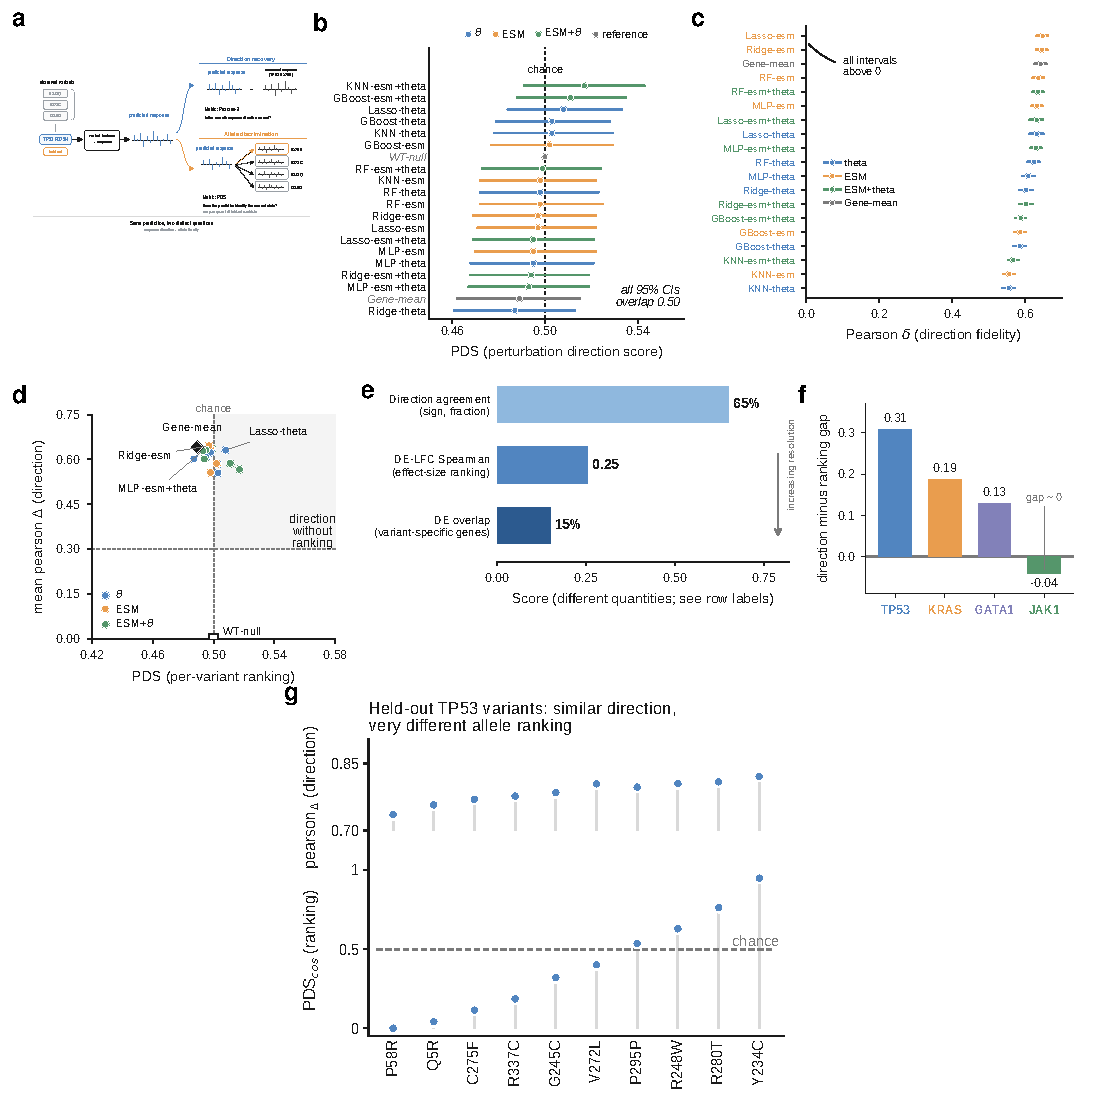
\includegraphics[width=\textwidth]{figures/fig2.pdf}
\caption{\textbf{Feature-based predictors recover gene-shared direction without reliable allele discrimination.}
\textbf{a}, How a held-out variant is scored: the predicted response is evaluated for direction recovery (Pearson-$\delta$) and, separately, for allele discrimination (PDS, whether it identifies its own variant among all candidate variants of the same gene, training and held out; Methods).
\textbf{b}, Allele-level PDS-cosine for 20 predictors; whiskers are 95\% bootstrap intervals over held-out variants, and all 19 non-null intervals overlap the chance level of 0.50.
\textbf{c}, The same predictors recover perturbation direction (Pearson-$\delta$), intervals as in \textbf{b}. A separate null axis carries zero, so the broken main axis resolves the confidence intervals, whose bounds span 0.54 to 0.66 around point estimates of 0.55 to 0.65, while all 19 non-null intervals stay visibly above zero.
\textbf{d}, Methods cluster in the direction-without-ranking regime.
\textbf{e}, Biological resolution falls along the ladder from gene-shared to allele-specific: programme direction 65\% (64 to 66\% across the 18 in-house heads, chance 50\%), effect-size order DE-LFC Spearman 0.25 (0.24 to 0.27, null 0), responding-gene identity 15\% DE overlap (13 to 16\%).
\textbf{f}, The two axes per gene, shown side by side rather than subtracted because their nulls differ; small points are the 18 in-house heads and diamonds their mean (Pearson-$\delta$ 0.77, 0.68, 0.58 and 0.41; PDS-cosine 0.46, 0.50, 0.46 and 0.45 for TP53, KRAS, GATA1 and JAK1).
\textbf{g}, Per-variant scores (Ridge-esm, TP53) show stable direction but unstable ranking; each of the 59 variants is the mean over the splits holding it out (84 evaluations; median Pearson-$\delta$ 0.80, median PDS-cosine 0.37).
\textbf{h}, The 20 predictors of \textbf{b} and the five published models of Fig. 3g, 25 in total, scored after the gene-shared programme is removed with a training-variant mean. Chance on this axis is 0.524, not 0.50 (amber). Filled, the six above their own permutation null.}
\label{fig:2}
\end{figure}


\subsection*{Allele-ranking failure persists across metrics, representations and model interfaces}

A chance-level ranking floor could in principle be manufactured by the evaluation instead of encountered in the measurement. If evaluation design set the floor, varying the generalization split should lift PDS; it did not. Across five of the six generalization splits (the sixth, cross-gene, is defined but excluded from the main grid because the datasets do not share a gene space, Methods), the two evaluation axes moved independently of each other. Pearson-$\delta$ stayed positive under the random, positional-extrapolation and compatibility splits, typically between 0.55 and 0.75, and fell mainly under mechanistic extrapolation and low-depth evaluation (Fig. 3a,b). PDS, in contrast, remained inside the empirical chance regime under every split (Fig. 3a,c), degrading most under low-depth evaluation. No split produced a consistent above-chance allele-discrimination regime, so the direction-ranking dissociation is not a property of the random holdout setting.

Neither the geometry of the distance function nor the unit of aggregation moved that verdict. Cosine, L1 and L2 distances gave nearly identical PDS distributions across the 18 feature-model combinations, all clustered at the chance level of 0.50 (Fig. 3d). Resolving the same grid by gene and split instead of by method reproduced the pattern (Fig. 3f): Pearson-$\delta$ exceeded PDS in 15 of 17 combinations, the two exceptions both arising in small held-out mechanistic-extrapolation sets, the KRAS set where the metrics nearly coincided (0.71 versus 0.72) and the JAK1 set where direction recovery itself collapsed (Pearson-$\delta$ = 0.02). The lowest value in the grid, a PDS of 0.19 in the GATA1 low-depth split, already anticipates the depth-dependent detection limit quantified below.

Preprocessing choices were equally unable to lift the floor. Refitting the per-gene standardization on training variants and wild-type cells only, excluding every held-out variant, left all predictors at or below chance (no method above 0.50; mean $\Delta$PDS $=-0.01$ against the reported all-cell standardization) with direction recovery unchanged, so the transductive standardization used throughout is, if anything, conservative with respect to the null (Supplementary Note).

Richer variant encodings did not close the gap either. Under identical splits, heads and scoring, the six-dimensional biophysical $\theta$ vector was compared with 1,280-dimensional ESM-1v embeddings, modern ESM2 embeddings\cite{ESM2}, three mutation-aware ESM2 constructions that encode the change relative to wild type (the mutant-minus-wild-type global embedding, the mutated-residue hidden-state difference and a local-window difference), and AlphaMissense\cite{AlphaMissense}, a purpose-built structure- and evolution-informed variant-effect predictor. Every representation left allele discrimination at chance (PDS 0.46 to 0.47, single-draw estimates that sit marginally below the 15-subsample values of Fig. 2 but carry the same chance verdict), with similar direction recovery throughout (Pearson-$\delta$ 0.63 to 0.66; Fig. 3e, Supplementary Note).

Three controls localize where this discrimination failure does and does not originate. The direction channel was not feature-driven: the featureless predictor that outputs the training gene mean already reached Pearson-$\delta$ 0.66 in this single-draw control, and shuffling the ESM2 features across variants within a gene left PDS at chance. Nor did the representation discard the mutation: the mutated-residue difference was highly variant-specific, with within-gene distances 91\% of between-gene distances against 0.1\% for the gene-identity-dominated global embedding, yet it too failed. And AlphaMissense pathogenicity did not track the measured transcriptional effect size in the three genes carrying enough scored variants to estimate the association (Spearman $-0.08$, $-0.05$ and $0.09$ for TP53, KRAS and GATA1, at $n = 84$, 78 and 201). In JAK1 only 11 of 26 variants are scored and the point estimate of $0.41$ is not significant ($P = 0.21$), so that gene neither supports nor excludes an association (Supplementary Note, Supplementary Table 4). The floor therefore does not originate in the input. Whether it originates in the model interface, in the mapping from features to responses, or in the ground-truth measurement is taken up in turn, first for published models and their interfaces below, then for the measurement itself (Fig. 4, Fig. 5).

Published perturbation-prediction models occupied the same regime once re-scored through a single harness: the same held-out variants, pseudobulk profiles, tie-aware PDS, and the bootstrap and permutation controls used for the in-house heads (Fig. 3g, Supplementary Table 4; Methods). Four of the five variant-conditionable models that ran to completion remained at chance: scGen (PDS 0.49, 95\% CI 0.46--0.52), scVIDR (0.50, 0.48--0.53), Biolord (0.49, 0.47--0.52) and CellFlow (0.51, 0.48--0.54); the fifth, PerturbNet, is taken up below. One of the four is scored on part of the benchmark rather than all of it: the scVIDR re-implementation returned non-finite predictions for every JAK1 variant, so 59 of its 518 held-out evaluations (11.4\%, four of 17 gene-by-split cells) carry the harness's chance value for an unscorable prediction rather than a measurement. Excluding those cells instead of scoring them at chance moves its estimate from 0.504 to 0.505, so the verdict does not turn on the convention, but the model is at chance on three genes and absent on the fourth (Methods). None exceeded the feature-model baselines of Fig. 2, whose intervals also overlapped chance, so for the evaluated variant-conditionable models allele discrimination remains unresolved.

The remaining public tools either cannot represent the task or do not clear it. scGPT, GEARS and STATE key their perturbation representation to the identity of the perturbed gene, so these gene-keyed models are allele-blind by construction: all variants of a gene collapse into one prediction, and only 4 of 470 variants (0.85\%) are representable at all (Fig. 3h). What such a collapse scores is shown by the Gene-mean reference, gene-constant by construction, which sits at chance (PDS 0.49). A compositional autoencoder (CPA) fitted with a variant-feature encoder did not converge on the continuous inputs (Supplementary Note). One generative flow, PerturbNet, marginally exceeded the analytic 0.50 chance level (PDS 0.54), but its predictions are confined to a 50-dimensional expression subspace in which random vectors already score 0.52; its exceedance over a permutation null estimated inside that subspace was not significant (permutation $P=0.13$), and its direction recovery was negligible (Pearson-$\delta$ 0.13). The subspace controls therefore leave this single marginal point uninformative about allele discrimination.

Across this section, five model classes compatible with continuous variant inputs were scored on the task, feature regression, latent arithmetic, disentanglement, optimal transport and conditional-flow generative models, and none achieved above-chance allele discrimination, while gene-keyed foundation models could not be scored at all, an interface incompatibility rather than a performance failure. The chance-level verdict thus persists across every model class that can express an allele, and across changes of split, distance geometry, standardization and input representation, which argues against a failure local to any single architecture. With evaluation design, input representation and model interface all excluded, the remaining question is whether the experimental ground truth reproducibly encodes allele identity.


% printed Figure 3; build artifact keeps its original basename
\begin{figure}[htbp]
\centering
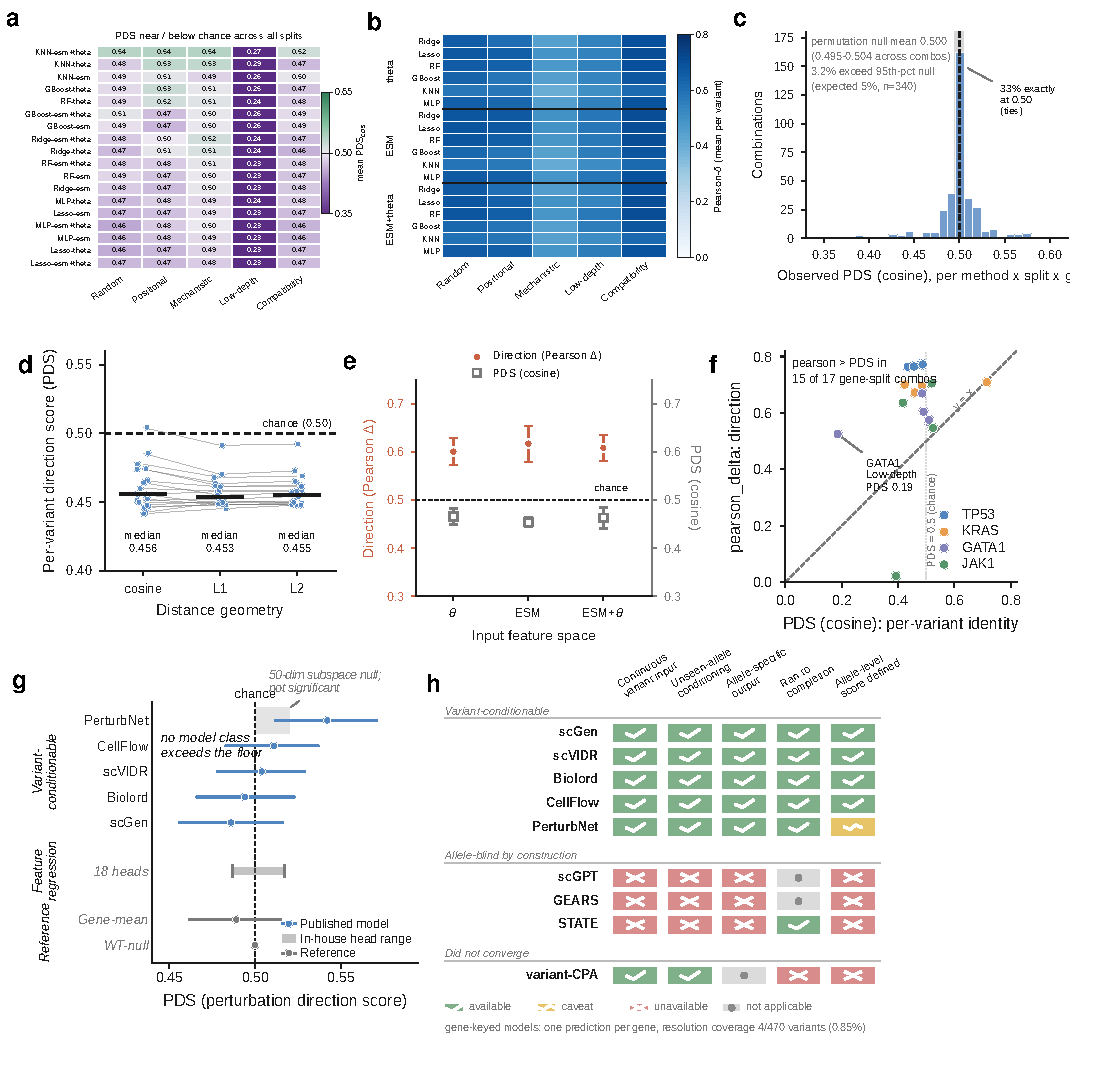
\includegraphics[width=\textwidth]{figures/fig4.pdf}
\caption{\textbf{Allele-ranking failure persists across evaluation choices and model interfaces.}
\textbf{a}, PDS across five generalization splits stays near chance, with no split showing a consistent above-chance allele-discrimination regime and the strongest collapse under the low-depth split.
\textbf{b}, Pearson-$\delta$ stays consistently positive across the same splits.
\textbf{c}, Empirical permutation null: within-split label permutation centres PDS at 0.50 (per-combination null means 0.495--0.504), with observed exceedances of the 95th percentile at 3.2\% (consistent with chance), so chance-level PDS is not an artefact of the analytic baseline.
\textbf{d}, Ranking failure is invariant to the distance function (cosine, L1 and L2 all near chance across the 18 feature-model combinations).
\textbf{e}, Richer features do not close the ranking gap ($\theta$, ESM and ESM+$\theta$ all near 0.50); error bars are s.d. over the six model heads.
\textbf{f}, The dissociation holds across all gene-by-split combinations, with Pearson-$\delta$ exceeding PDS in 15 of 17.
\textbf{g}, Published perturbation models scored under one identical harness (same held-out variants, pseudobulk profiles, tie-aware PDS and bootstrap/permutation controls): every variant-conditionable model except PerturbNet, the in-house feature-regression range and both references overlap the PDS = 0.50 chance line; PerturbNet's full-harness estimate exceeds 0.50, but random predictions confined to its 50-dimensional output subspace already reach an elevated PDS, and its in-subspace exceedance over the corresponding permutation null is not significant ($P=0.13$) (Supplementary Table 4).
\textbf{h}, Interface-compatibility audit: gene-keyed models (scGPT, GEARS, STATE) are allele-blind by construction, resolving only 4 of 470 variants (0.85\%); this is interface incompatibility, distinct from performance failure.}
\label{fig:3}
\end{figure}
\subsection*{Split-half and sibling diagnostics identify measurement-limited regimes}

One alternative remains: predictors may fail to rank alleles not because the models are wrong but because the ground-truth variant responses are not stably separable at the available depth. We therefore located each dataset on the three nested levels introduced above, detection, identification and prediction, each a precondition for the next (Supplementary Table 3).

Detection was quantified first, directly on the single-cell distributions rather than on the pseudobulk prediction target (Fig. 4a,b). For each variant, cells were randomly divided into two halves, and the energy distance between the two halves of the same variant (D\_self) was compared with the distance between that variant and wild type (D\_null). A D\_self/D\_null ratio near 1 indicates that within-variant sampling variation is comparable to the variant-to-wild-type signal, so the detection window is closed; a ratio well below 1 indicates an open window, in which the perturbation effect stands above sampling noise.

The four datasets occupied distinct detection regimes (Fig. 4c). TP53 (D\_self/D\_null = 0.96, 95\% CI 0.95--0.98), KRAS (1.00, 0.99--1.02) and GATA1 (0.88, 0.85--0.90) sat near the floor, whereas JAK1 was well separated from it (0.21, 0.12--0.33), reproducing the ordering seen in the direction-ranking dissociation of Fig. 2f. This per-dataset gradient describes the measurement regimes available here rather than an intrinsic property of the proteins. For the three low-effect datasets detection was at best marginal: the variant-to-wild-type shift is comparable to within-variant replicate noise, and under the split-half criterion almost no variant clears the per-variant floor at any evaluated depth (Fig. 4g); clearing it would in any case license no claim about alleles.

Identification, the stricter level that actually bounds allele benchmarking, then failed. A model-free classifier trained to separate the single cells of two sibling variants under cross-validation was at chance for TP53 and KRAS and near chance for GATA1 (median identification AUROC 0.49, 0.50 and 0.52, against 0.50 under label permutation and a wild-type-versus-wild-type control), rising only for JAK1 (0.87; Fig. 4e). Distributional distances agreed: the transcriptional distance between sibling alleles fell below within-variant replicate noise for almost every pair in TP53, KRAS and GATA1 (median nearest-sibling cosine distance 0.23 to 0.46 versus replicate noise near 0.97), leaving 0\%, 0\% and 3.8\% of allele pairs resolvable, whereas the threefold-lower replicate noise of JAK1 left 78.5\% resolvable (Fig. 4d; at the single-nearest-sibling level JAK1 identification is a benchmark-level rather than a per-variant property). The GATA1 measurement therefore sits between these outcomes: detection is marginal, the pairwise signal is weak, and no sibling allele is reliably recovered as a variant's nearest neighbour.

Detection and identification degraded together across these datasets, but they remain distinct levels: detection-level rankability, the split-half signal-above-replicate-noise criterion used for Fig. 4g,h and for the atlas comparison below, is necessary but not sufficient for identification, and a dataset can clear detection while still leaving a benchmark nothing to score. The identification verdict was invariant across five distance families, from energy and maximum-mean-discrepancy to sliced-Wasserstein, cosine and Euclidean, so it is not an artefact of energy-distance geometry (Supplementary Note). It is equally not an artefact of the pseudobulk prediction target: the classifier and these distributional distances operate on the single cells themselves, so the discrimination floor is present in the full response distributions and not only in averaged profiles (Supplementary Note).

Effect size and depth taken together show why the effect-size-to-noise window, rather than cell number, sets the floor (Fig. 4f,g). JAK1 had the lowest nominal depth among the four (median 104 cells per variant) but the widest effect-size-to-noise window, and it was already saturated in the split-half detection assay at 50 cells per half. TP53 and KRAS were profiled far more deeply yet had narrow allele-specific effect windows, remaining close to the noise floor at median raw depths of 929 and 1,000 cells per variant. Subsampling from 30 to 150 cells per half in the canonical PCA-50 space preserved the same ordering, over a cohort held fixed within each gene at the variants evaluable at the deepest rung so that every depth refers to the same variants. TP53 and KRAS stayed at 0\% detectable at every depth and GATA1 reached only 3.8\% at the deepest rung, whereas JAK1 was already 83\% detectable at 30 cells per half and fully detectable from 50 onwards. Within this tested range, additional cells left TP53 and KRAS unchanged, moved GATA1 by under four percentage points, and left JAK1 already saturated. Depth is therefore not the quantity to optimize when the allele-specific effect is small relative to sampling and biological variability, a statement about the assays and protocols evaluated here rather than a depth requirement that transfers to other measurements.

At native depth, and scored over every perturbation and not over matched subsamples by the direct split-half energy-distance definition, the ordering persisted: the three low-effect allele-level datasets (TP53, KRAS and GATA1) were 97.6--100\% un-rankable by this detection-level criterion, whereas JAK1 remained a positive control with only 10\% un-rankable variants (Fig. 4h). Results were qualitatively robust under alternative rankability criteria, including bootstrap-CI-based, increased-stringency and ratio-threshold definitions (Supplementary Fig. 1). The same detection-level floor was also present in external gene-level Perturb-seq atlases, motivating the prospective design analysis below: finite-depth distributional distances can leave a substantial fraction of individual perturbations below the resolution required to score them, in gene- and drug-level screens as well as in allele data. This per-perturbation floor is distinct from the benchmark-level ranking resolution examined next, to which many individually detection-unrankable perturbations can still contribute in aggregate (Fig. 5).

Read across the detection, identification and prediction levels, these diagnostics locate each dataset on a solvability map. As measured here, TP53 and KRAS are measurement-limited: allele identity is not reproducibly encoded at the available depth, so a benchmark built on them cannot reward an allele-specific prediction. GATA1 lies at the boundary of the same regime. JAK1 is identifiable under its assay and protocol, which makes it the only dataset here in which an allele-level score reports on the model rather than on the measurement. What remains is to quantify how much allele discrimination the measurement itself permits, and what follows for the benchmark when that quantity sits at the floor.


% printed Figure 4; build artifact keeps its original basename
\begin{figure}[htbp]
\centering
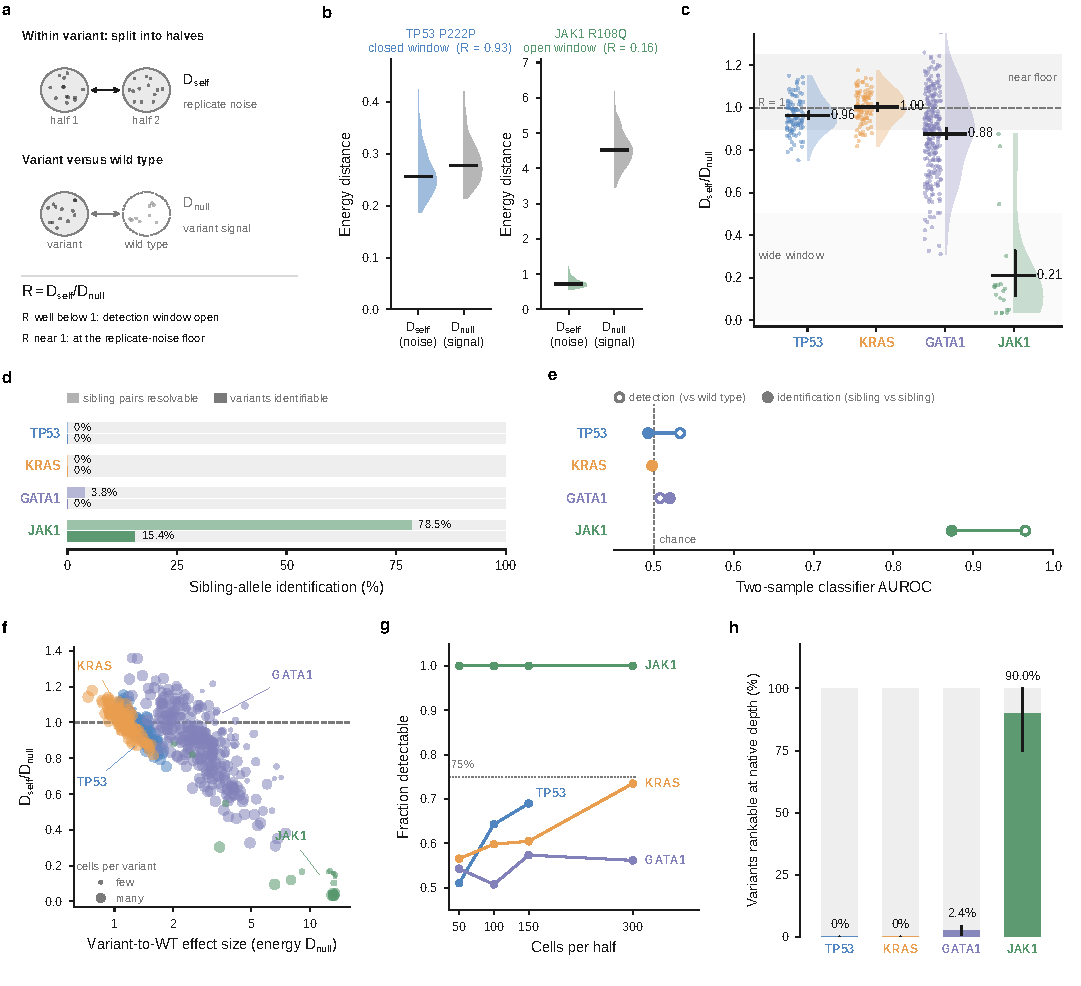
\includegraphics[width=\textwidth]{figures/fig3.pdf}
\caption{\textbf{Split-half analysis reveals a marginal detection window and absent allele identification.}
\textbf{a}, Definition of the detection window from within-variant ($D_\mathrm{self}$) and variant-to-wild-type ($D_\mathrm{null}$) distances.
\textbf{b}, Representative variants illustrate a closed window (TP53 P222P, $D_\mathrm{self}\approx D_\mathrm{null}$) and an open window (JAK1 R108Q, $D_\mathrm{self}\ll D_\mathrm{null}$); $R$ is a 200-seed split-half estimate for one variant, not the native-depth statistic of \textbf{c}, \textbf{f} and \textbf{h}; the sub-panels have independent y scales.
\textbf{c}, Per-variant $D_\mathrm{self}/D_\mathrm{null}$ places TP53 (0.96), KRAS (1.00) and GATA1 (0.88) near the detection floor and JAK1 (0.21) well below it; n = 98, 92, 254 and 20 variants (six JAK1 variants have too few cells to split), bar and whisker are the gene mean and its 95\% bootstrap interval, and the bands mark ratios 0.90--1.25 (replicate-noise floor) and 0--0.50 (window open).
\textbf{d}, Allele identification: the fraction of sibling-variant pairs whose transcriptional distance exceeds within-variant replicate noise (TP53 and KRAS 0\%, GATA1 3.8\%, JAK1 78.5\%) and the stricter fraction whose single nearest sibling is separable (JAK1 15.4\%, 0\% for the other genes).
\textbf{e}, Classifier two-sample test: cross-validated AUROC separating the single cells of sibling variants (identification) is at chance for TP53 and KRAS (0.49, 0.50), near chance for GATA1 (0.52) and high for JAK1 (0.87); detection against wild type (open symbols) follows the same ordering; label permutation gives 0.50.
\textbf{f}, Effect size and effective depth jointly determine the window, not cell number alone.
\textbf{g}, Depth titration in the canonical PCA-50 space at 30, 50, 100 and 150 cells per half, scored by the same $S>W$ criterion as \textbf{h} over a cohort held fixed within each gene at the variants evaluable at the deepest rung (n = 87 TP53, 91 KRAS, 157 GATA1 and 6 JAK1 variants): JAK1 is 83\% detection-rankable at 30 cells and saturated from 50 onwards, whereas TP53 and KRAS stay at 0\% at every depth and GATA1 reaches 3.8\%; whiskers are 95\% Wilson intervals.
\textbf{h}, Fraction of variants detection-rankable at native depth, i.e.\ split-half signal above replicate noise (TP53 0\%, KRAS 0\%, GATA1 2.4\%, JAK1 90\%; same n as \textbf{c}); whiskers are 95\% bootstrap intervals over variants, degenerate at exactly 0 and 100\%.}
\label{fig:4}
\end{figure}


\subsection*{The replicate ceiling separates measurement-limited from model-limited datasets}

With a ground-truth resolution floor established, two questions follow. How much allele discrimination can the measurement support, and can a benchmark at that resolution recover the true ordering of models? The first question needs a reference point that is measured, not assumed, so we scored an oracle predictor whose prediction for each held-out variant is an independent second measurement of that same variant, taken from a disjoint split-half pseudobulk and passed through the identical harness (Fig. 5a; Methods). The resulting quantity is the replicate ceiling, an empirical reproducibility reference at the available depth and protocol: it states how closely one measurement of an allele agrees with a second measurement of the same allele, which is the most that a benchmark scored against that measurement can reward. For TP53 and KRAS this reference was itself at chance (PDS 0.485, 95\% CI 0.445--0.525, and 0.500, 0.440--0.566). Split-half depth was not the explanation: the value was unchanged when all cells were used (0.486 and 0.492), and a near-true prediction, the deep true mean of a variant scored against the benchmark's own noisy measurement, also remained at chance (0.49 and 0.49; Supplementary Note). In these two datasets the replicate ceiling, the best feature-regression head (a maximum over 18 models, upward-biased under the null) and the near-true-prediction control are all statistically indistinguishable from 0.50 with overlapping 95\% confidence intervals. Above-chance allele discrimination therefore could not be reliably demonstrated at this resolution, and the reason is specific: the measurement cannot reliably reward even an essentially correct answer, so the binding limit lies in the resolution of the ground truth rather than in model capacity.

The replicate ceiling was not at the floor everywhere, and its spread across datasets separates two regimes that a model score on its own cannot distinguish. GATA1 sat marginally above chance (0.572, 0.549--0.595), consistent with its small resolvable-pair fraction and with the marginal detection window above. In the JAK1 dataset, by contrast, the ceiling reached 0.792 (0.742--0.838) while the best in-house model stayed near chance (0.52), so the measurement there is adequate for allele discrimination and the shortfall is computational; the best score attainable inside that family's own prediction span was 0.690 (0.638--0.742), so its shortfall is not forced by the geometry of the evaluation (Fig. 5b,c, Supplementary Table 5, Supplementary Note). That regime is evaluable, in that the ground truth can reward an allele-specific prediction, but unresolved: none of the predictors evaluated here approached the replicate ceiling under the available assay and protocol. The more favourable JAK1 window is a property of that per-dataset measurement regime rather than evidence of stronger allele biology. The ceiling has a defined scope of its own. It is an empirical reproducibility estimate at the available depth and protocol, not a mathematical upper bound on all denoising or hierarchical models: a model that pooled information across variants could in principle exceed a single replicate, although the benchmark as measured could not reward it.


\subsection*{Benchmark ranking resolution collapses at the floor and is non-monotone above it}

The second question is different in kind, and the distinction is easy to lose. Whether an individual perturbation is separable from its siblings is a per-perturbation property of that perturbation's effect size and noise; whether a benchmark can order competing models is a property of the perturbation set as a whole, and the two need not agree. To probe the set-level property we built synthetic predictors of known, graded quality by interpolating between the gene-mean profile and each variant's measured effect (Fig. 5d), then asked how often the observed PDS recovered their true ranking under bootstrap resampling of the held-out variants (Methods). When the replicate ceiling was at or near chance ($\leq 0.52$, comprising TP53, all evaluated KRAS depths and the shallowest GATA1 configuration), the true predictor order was recovered only 27\% of the time and the best predictor selected only 38\% of the time, far from reliable. Once the window opened modestly across the evaluated GATA1 depth configurations (ceiling 0.52--0.55), correct ordering rose to 95\% and correct winner selection to 97\%; above a ceiling of 0.65 both approached 1.0 (Fig. 5g). These transition points are empirical to the present candidate-set sizes and distance metric rather than fixed thresholds, and recovery also fell when few variants were held out, as expected from test-set size. The rise is also not indefinite: on configurations in which the measurement resolution was dialled continuously, ordering recovery peaked near a ceiling of 0.705 and declined above it, because two predictors that both reach the ceiling become mutually indistinguishable whatever their true quality (Methods). TP53, KRAS and GATA1 lie below that peak, whereas JAK1 and the six external screens of Supplementary Table 9 lie above it and still recovered the ordering with probability 0.90 or higher, so the decline appears in the dialled configurations and was not reproduced in the measured datasets; neither trend should be extrapolated. The consequence is a validity condition rather than a description: below this resolution a leaderboard is unstable whatever the models' true quality, so the ranking it prints reports the measurement as much as the methods (Fig. 5g).

Across benchmarks, this set-level resolution varies widely. We applied the same analysis to five diverse public perturbation benchmarks at a fixed shallow depth of 50 cells per half for comparability. Norman, Replogle, Adamson and the Virtual Cell Challenge training set\cite{VirtualCellChallenge2025} all recovered the true predictor ordering in every bootstrap resample of this construction (resolution 1.00; the frozen criterion of Supplementary Table 9 puts the same four datasets at 0.903 to 0.997) and a drug screen (sci-Plex\cite{SciPlex2020}) reached 0.77. TP53 and KRAS were the only datasets at the floor (0.01 and 0.02; Fig. 5f). Set-level ranking resolution and the per-perturbation detection-unrankable fraction of Fig.~6f are therefore separate quantities, and a dataset can score well on one while failing the other: an atlas such as Replogle can leave roughly half of its individual perturbations detection-unrankable and still order graded predictors, because many weak perturbations aggregate across thousands of interventions, whereas each allele dataset here contributes at most a few hundred. The same arithmetic works in the allele setting, where the many variants of GATA1 (0.51 at this shallow depth, versus 0.95 at its native ceiling in Fig. 5g) partly offset a low per-variant signal. The position of the allele datasets at the floor thus reflects a lower ground-truth resolution than that of diverse gene- and drug-level screens, rather than a peculiarity of the evaluation. Measurement resolution and benchmark ranking resolution converge on one conclusion for the field: allele-specific prediction cannot be judged from model scores alone, because the same score has different meanings in a measurement-limited and in a model-limited regime, and which regime applies is fixed by the measurement before any model is trained.


% FIGURE 5 (keystone: replicate ceiling -> benchmark validity)
\begin{figure}[htbp]
\centering
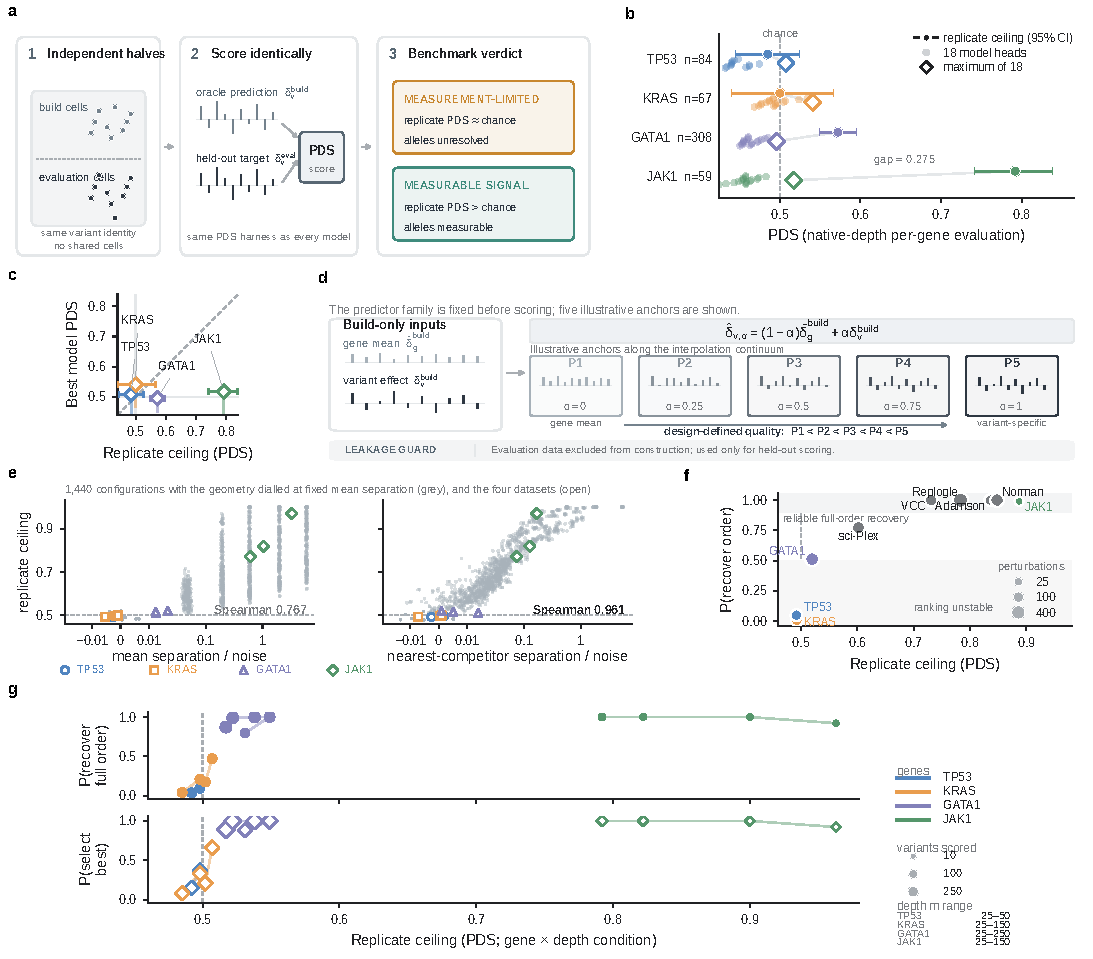
\includegraphics[width=\textwidth]{figures/fig5.pdf}
\caption{\textbf{The replicate ceiling governs attainable discrimination and benchmark validity.}
\textbf{a}, The oracle predictor: an independent second split-half measurement of each held-out variant, scored through the identical harness. This empirical replicate ceiling is a depth- and protocol-specific reproducibility reference, not a mathematical upper bound.
\textbf{b}, Replicate ceiling per gene (native depth) versus the best in-house model; whiskers are 95\% bootstrap intervals over held-out variants. TP53 and KRAS ceilings sit at chance (measurement-limited), and the best model's slight excess there is best-of-18 selection noise, its interval also covering 0.50. JAK1's ceiling is high while models stay near chance, a residual computational gap.
\textbf{c}, Ceiling-versus-model phase map: horizontal bars are 95\% bootstrap intervals on the ceiling, the vertical bar spans the 18 in-house heads, the diamond their maximum (a selected point estimate, no model interval implied); chance is the only threshold drawn. A ceiling whose interval covers 0.50 cannot score any model (TP53, KRAS). The shaded diagonal is the benchmark-solvable band, a model within 0.035 PDS of its ceiling; below it the ceiling clears chance but the model does not follow (GATA1, JAK1).
\textbf{d}, Synthetic predictors of graded quality built by interpolating between the gene-mean profile and each variant's measured effect, fixing the true ordering by design.
\textbf{e}, What orders the replicate ceiling: not the mean separation over pairs (left) but each variant's nearest competitor (right), both relative to sampling noise, symmetric-log axis. Grey, 1,440 configurations with the geometry dialled at fixed mean separation; open symbols, the four datasets at three depths (Methods).
\textbf{f}, Benchmark resolution across nine datasets: probability of recovering the graded predictors' true ranking versus each dataset's replicate ceiling (matched 50 cells per half). Four allele genes and five external screens trace a phase transition, collapsing at the floor (TP53, KRAS) and approaching one above $\sim$0.65; bands mark recovery $\geq$0.90 and $\leq$0.50 and are reading aids, not analysis thresholds, here and in \textbf{g}.
\textbf{g}, Full-order recovery and best-model selection are both low where the ceiling sits at chance (TP53, KRAS) and jump towards one once it clears 0.52 (GATA1) and beyond (JAK1); selecting a winner leads recovering the full order.}
\label{fig:5}
\end{figure}

\subsection*{Pilot measurements prospectively predict detection-level rankability}

If allele discrimination is meaningful only above a measurement floor, then which perturbations are evaluable has to be settled before any model comparison begins. Using leave-one-dataset-out (LODO) cross-validation across the four allele-resolved datasets assembled here and three external Perturb-seq atlases, we trained a rankability predictor whose single feature is each perturbation's pilot-estimable pseudobulk effect size (Fig. 6a; Methods).

A single effect-size feature was sufficient to separate detection-rankable from detection-unrankable perturbations. Across the five datasets in which rankability is non-degenerate, it did so with a mean AUROC of 0.96 (Replogle 0.97, Norman 0.93, Adamson 0.93, GATA1 0.95, JAK1 1.00; ROC curves and 95\% bootstrap intervals in Fig. 6b,c). The TP53 and KRAS datasets could not be evaluated at all: at native depth every one of their variants is detection-unrankable, and that single-class outcome is itself the clearest available statement, that under the assay, cell context and depth of these experiments the measurements lie entirely below the detection floor.

Because the retrospective predictor draws its feature and its label from the same cells, we next tested it prospectively on cells that the pilot never saw. Pilot measurements of 25 to 50 cells per perturbation were used to predict rankability at higher depth on the disjoint remainder, again under leave-one-dataset-out cross-validation. Across the three benchmarks with balanced labels (Adamson, Norman and Replogle) the pilot predictor reached AUROC 0.85, 0.94 and 0.99 (mean 0.93), with near-diagonal calibration and a label-permutation null of 0.49; a training-free predictor using the pilot signal-to-noise ratio performed comparably (0.84 to 0.98 per dataset), and the result held when the pilot was restricted to 25 cells (Fig. 6d).

One boundary condition qualifies the triage. What the pilot estimates is perturbation-versus-reference separation, that is detection-level rankability, which is necessary but not sufficient for allele benchmarking: a perturbation can clear the detection floor and still lack the sibling-level separation that identification requires (Fig. 4d,e). Pilot rankability therefore excludes perturbations that are clearly unmeasurable rather than certifying that allele identity is recoverable, and it orders candidate perturbations relative to one another within a given assay rather than fixing a depth that transfers across assays.

Beyond triage, the same effect-size analysis recasts experimental depth as a quantity conditioned on effect size instead of fixed in advance (Fig. 6e). In the JAK1 dataset, whose measured responses are comparatively large under its assay and cell context, detection was already 83\% at 30 cells per half and saturated from 50 onwards, whereas the TP53 and KRAS measurements remained near the noise floor despite median raw depths of 929 and 1,000 cells per variant. The design target is therefore not a fixed cells-per-variant threshold, but the depth demanded by a particular combination of effect size, inter-variant difference and sampling noise. Calibrating that effect-size-to-noise window against the attainable discrimination makes the requirement quantitative, since sampling noise falls as the reciprocal of depth while the separation between perturbations does not change with it, so a pilot fixes the depth needed to reach a target (Methods). Applied to these datasets the calculator answers only where the pilot separation is significantly positive: for JAK1 it prescribes 10, 12 and 19 cells per group to reach a replicate ceiling of 0.7 from pilots at three different depths, an agreement within a factor of two across independent cell sets, and 55 to 99 cells to reach 0.9. For TP53 and KRAS at every depth, and for GATA1 at two of three, it returns nothing: their separation is estimated at or below zero, and no finite depth recovers a separation that is not there (Supplementary Table 7). Refusing is the correct output, since inverting a curve from an estimate whose interval covers zero produces a confident number and no information.

The same criterion, in its frozen, packaged form, was applied to six published screens, two new to this work and a third not previously scored by it. Every one fell below identification: detectable fractions ranged from 26\% to 90\% while identifiable fractions ranged from 0.5\% to 43\%, and no screen reached the majority-identifiable threshold the criterion requires (Fig.~6h, Supplementary Table 9; Methods).

How much the design framing matters is visible in the external gene-level atlases (Fig. 6f). At native depth, 55.3\% of perturbations were detection-unrankable in Replogle 2022\cite{Replogle2022} (95\% CI 52.8--57.5\%), compared with 14.6\% in Adamson 2016\cite{Adamson2016} and 3.4\% in Norman 2019\cite{Norman2019}. Comparing like with like, on the perturbations measured at both depths, normalizing to the same shallow depth (n = 50 per half) left every dataset less evaluable and moved the detection-unrankable fractions towards one another: Replogle rose from 52.0\% to 54.9\% (n = 1,299), Adamson from 14.6\% to 38.5\% (n = 96) and Norman from 2.7\% to 11.2\% (n = 224). Depth normalization can therefore change substantially which perturbations are evaluable, while dataset-specific effect-size structure remains important.

Taken together, these analyses point to design principles, not a fixed protocol, each measurement gate licensing a different report (Fig. 6g): detection permits a claim about a perturbation against its reference, and identification permits an allele-level claim. Perturbations that fall below the detection floor are better redesigned, measured more deeply, or reported separately, than entered into a model comparison their ground truth cannot arbitrate. Evaluation at allele resolution is therefore better organized as a power-aware, stratified design over perturbations than as a uniform ranking of models.

% FIGURE 6
\begin{figure}[htbp]
\centering
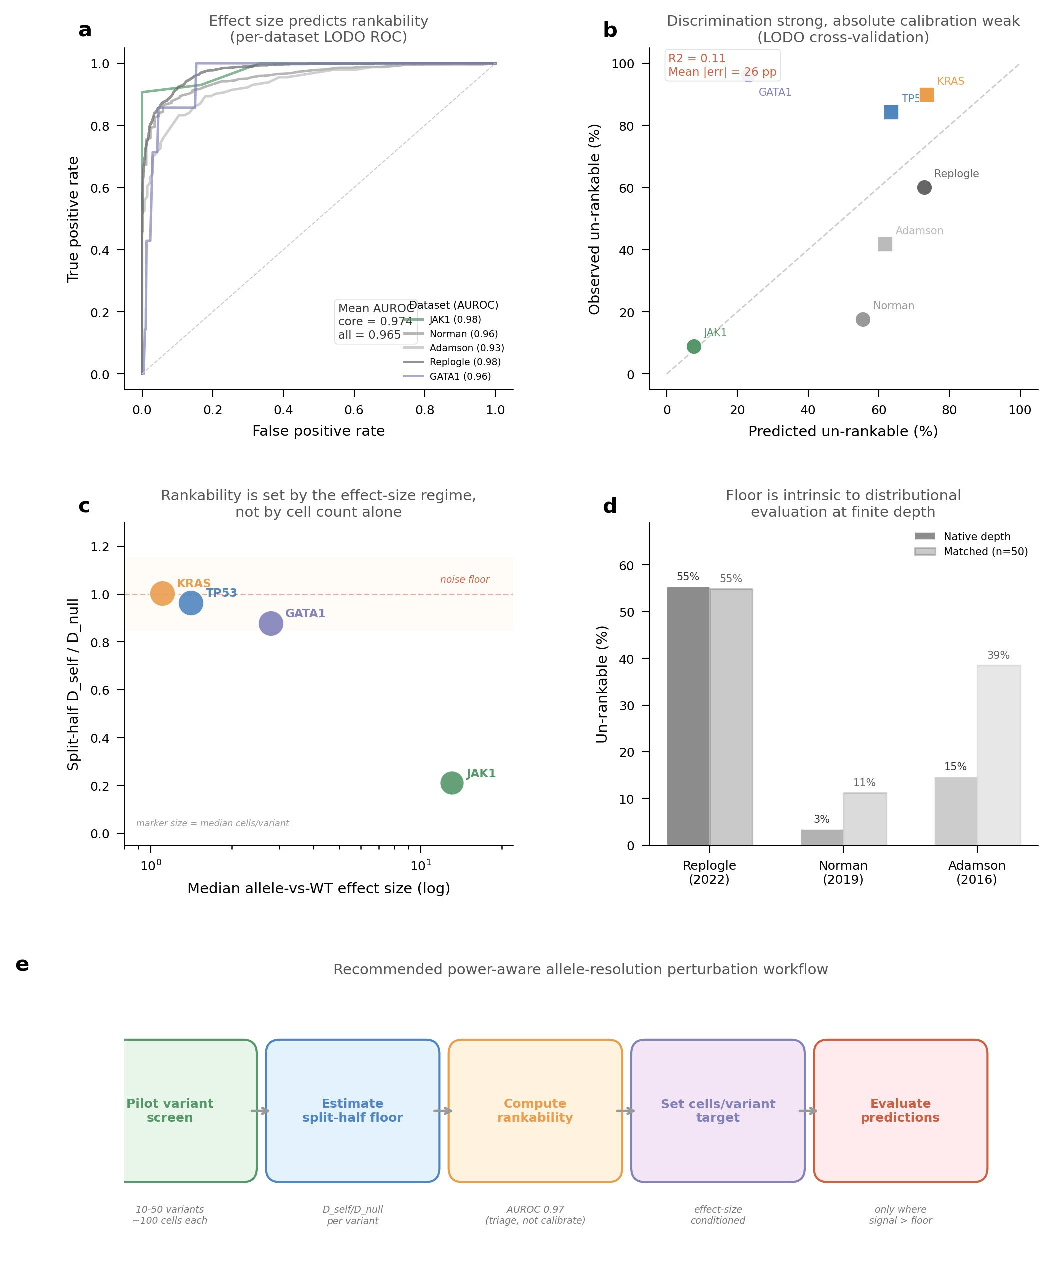
\includegraphics[width=\textwidth]{figures/fig6.pdf}
\caption{\textbf{A power-aware reporting protocol for allele-resolution perturbation prediction.}
\textbf{a}, Rankability prediction: each perturbation's pilot-estimable effect size triages which perturbations clear detection-level rankability before any model comparison begins.
\textbf{b}, Leave-one-dataset-out ROC curves of the single-feature (log effect-size) rankability predictor. This arm is retrospective: predictor and label are estimated from the same source cells. TP53 and KRAS are single-class and are not drawn.
\textbf{c}, Dataset-level LODO AUROC (mean 0.96): Replogle 0.97, Norman 0.93, Adamson 0.93, GATA1 0.95, JAK1 1.00; whiskers are 95\% bootstrap intervals over held-out perturbations. TP53 and KRAS are uniformly detection-unrankable at native depth, so their AUROC is undefined.
\textbf{d}, Prospective validation: from a 25 to 50-cell pilot, rankability at higher depth is predicted on disjoint held-out cells under leave-one-dataset-out cross-validation (AUROC 0.85, 0.94 and 0.99 for Adamson, Norman and Replogle; a label-permutation null gives 0.49), with near-diagonal calibration. Intervals are 2,000 perturbation bootstraps and calibration bars are Wilson 95\% intervals over bins of about 100 perturbations.
\textbf{e}, Effect-size-conditioned design landscape: detection-rankability is set by the effect-size regime, not by a fixed cell-count cutoff (filled, rankable; open, un-rankable).
\textbf{f}, Native versus depth-matched (n = 50 per half) detection-unrankable fraction on external gene-level atlases, paired over the perturbations measured at both depths (n = 1,299, 96 and 224); thin bars are Wilson 95\% intervals. All three become less evaluable at matched depth (Replogle 52 to 55\%, Adamson 15 to 39\%, Norman 3 to 11\%).
\textbf{g}, Nested measurement gates and the report each one licenses: detection permits a claim about a perturbation against its reference, identification permits an allele-level claim, and a perturbation below the floor is reported separately rather than as a model failure.
\textbf{h}, The same criterion, frozen before use and applied without per-dataset tuning to six published screens (Methods). Detectable against identifiable fraction at 50 cells per group; marker area, perturbations scored; dashed line, equality. None reaches identification.}
\label{fig:6}
\end{figure}

\section*{Discussion}

Allele-specific prediction is not gene-level prediction at finer resolution: recovery of a shared perturbation programme and identification of the causal variant are separable objectives, and the evaluated predictors met the first while failing the second, reproducing the transcriptional direction associated with perturbing a gene while carrying little information about which coding variant produced that response. Two controls fix how that correlation should be read. A featureless gene-mean baseline, which by construction assigns every variant of a gene the same profile, already reached the direction score of the best feature-based model, so that channel is available without any allele information at all. And when each measured effect was decomposed into a gene-shared component and an allele-specific residual, direction recovery on the residual was near zero, so removing the shared programme removed the recovered signal. Scoring discrimination on that residual against its own calibrated null, six of 25 methods exceeded that null by between 0.011 and 0.025 and none survived correction for the 25 tested, so any recoverable allele-specific signal in these heads is bounded at a few points of discrimination and none is established. Allele-level prediction must consequently be defined jointly by the mapping from variant features to cellular response and by the resolution of the measurement used to evaluate that mapping.

Read through the detection, identification and prediction hierarchy, the four datasets did not fail in the same way, and the distinction they draw is between measurement-limited and model-limited regimes. TP53 and KRAS are measurement-limited, their replicate ceiling itself indistinguishable from chance, and GATA1 sits just above that floor rather than across it. Only the JAK1 dataset cleared identification, and there an independent second measurement of the same variants recovered allele identity that none of the evaluated predictors recovered from molecular features, so JAK1 defines an evaluable but unresolved, model-limited regime rather than evidence that allele-level prediction is intrinsically impossible. The task is therefore not uniformly out of reach: which solvability state a dataset occupies is an empirical property that can be established before any model is compared.

Benchmarks that treat experimentally derived response profiles as fixed ground truth place uncertainty primarily on the model\cite{AIVirtualCell2024,scPerturb,Pertpy,PerturBench}, and rankings already depend on baseline choice, systematic variation and metric geometry\cite{AhlmannEltze2025,Systema}. Measurement resolution is a further and logically prior source of uncertainty: a measured profile is an estimate, not a noiseless label, so a task's resolution has to be established before models are ranked on it. Benchmark design should accordingly distinguish two resolutions: perturbation-level resolution, whether individual interventions are reproducibly separable, and benchmark-level ranking resolution, whether the perturbation set as a whole can recover differences among predictors. Applied in its frozen, packaged form, the criterion placed none of six published screens above identification at 50 cells per group, the two largest gene-level atlases being 68.7\% and 51.2\% detectable against 0.5\% and 1.4\% identifiable (Fig.~6h). Three of its four pre-registered predictions were confirmed and one was not: the packaged criterion places Adamson 3.3 percentage points below Replogle in detectable fraction, reversing the order this manuscript's own pipeline gives, so the two agree on the extremes but are not interchangeable at the level of individual fractions (Supplementary Table 9). Those same two atlases recovered the ordering of graded predictors with probability 0.997 and 0.96 in that same packaged run, whereas two panels of seven and ten perturbations, which had the highest identifiable fractions in the set, recovered it with probability 0.11 and 0.42. Per-perturbation resolution and set-level ranking resolution therefore come apart in both directions, and neither substitutes for the other.

Experimental design and computational evaluation are therefore coupled, not sequential, concerns. Whether sibling alleles are resolvable was set here by effect magnitude, inter-allele separation and sampling noise rather than by nominal cell depth, and is plausibly shaped as well by biological heterogeneity, variant assignment quality, cellular context and stimulation, sampling time point and readout modality, none of which was varied across these datasets. Where depth is not the binding constraint, allele-resolved studies may need more informative designs: biological replication, improved variant assignment, matched stimulation, responsive cell states, time-resolved sampling, or orthogonal readouts of chromatin state, protein abundance, signalling activity and phenotype. Model design faces the mirror-image constraint: more expressive protein representations cannot compensate for an unresolved transcriptional target, and a resolvable target does not guarantee that current sequence- or feature-based models capture the context-dependent mapping from molecular variation to cellular response.

Several limitations bound these conclusions. The publicly available allele-resolved datasets cover only four genes, spanning three technologies and three cell contexts, so gene identity is partly confounded with measurement regime and cellular context, and the observed differences must be read as dataset-specific measurement regimes, not as intrinsic rankings of allele biology. The model-limited verdict rests on a comparatively small JAK1 panel: 26 variants in total, 20 entering the native rankability analysis, 14 at the matched 50-cell depth, and 9, 6 and one variant at the successively deeper titration levels. The prospective pilot analysis predicts detection-level rankability, that is, resolution of a perturbation against its reference, which is necessary but not sufficient for a power calculation on within-gene allele identification. The replicate ceiling is an empirical reproducibility reference for a specified depth and scoring protocol, not a mathematical upper bound on all denoising or hierarchical models. Pseudobulk profiles are the prediction target throughout, and although cell-level classifier controls show that the identification floor is not an artefact of averaging, pseudobulk evaluation may still underrepresent effects confined to rare subpopulations or shifts in cell-state composition. Transcriptomic response is also not the whole phenotype: alleles that are indistinguishable in expression space may still differ in protein state, signalling activity or organismal consequence. The model side is bounded as well: the compositional autoencoder did not converge, the gene-keyed foundation models were not scorable at all (4 of 470 variants representable), and 11.4\% of scVIDR's held-out evaluations carry the harness's chance value in place of a measurement. PerturbNet, the only model above 0.50, is set aside on a permutation test that is itself non-significant at $P = 0.13$, which is absence of evidence rather than evidence of absence. Controlled studies profiling multiple genes within shared experimental contexts, with biological replicates, depth titrations and multimodal readouts, will be needed to establish identification-aware power criteria.

Read together, these results support a measurement-aware principle for predictive cellular modelling: model performance is interpretable only at biological resolutions that the experiment itself can reproduce. Predictors should be judged on whether they recover allele-specific residual structure, not the gene-shared response that dominates direction-based scores, and allele-resolved experiments should establish identification before prediction is scored at all. The same requirement extends beyond coding variants to drug analogues, dose series, combinatorial perturbations and multimodal phenotypes, wherever closely related interventions must be told apart rather than merely detected. By separating what is shared across variants from what identifies an allele, and what is unmeasured from what remains unmodelled, this study provides a foundation for deciding when allele-specific cellular prediction is scientifically testable.


\section*{Methods}

\subsection*{Study design}

This study is a retrospective evaluation of held-out protein-coding variant prediction from single-cell perturbation data, with AllelePerturb as its task formalization and evaluation protocol. All data are publicly available single-cell perturbation datasets, and no new human, animal or biological samples were generated. The primary unit of prediction and of statistical resampling is the protein-coding variant condition. Throughout, \textit{allele} denotes this experimentally assigned protein-coding variant condition rather than a phased genomic haplotype.

Four genes (TP53, KRAS, GATA1 and JAK1) assayed by three technologies (Perturb-seq, base editing and scSNV-seq) were included. To our knowledge, these are the publicly available single-cell perturbation datasets that resolve individual protein-coding variants with reusable per-variant labels. All eligible variants and cells were used, so sample size was not predetermined.

For each generalization split, models were trained on the training variants of a gene and evaluated on its held-out variants. Every model was scored through a single evaluation harness. The primary analyses quantify transcriptional direction recovery and within-gene allele discrimination. Separate replicate-based analyses assess perturbation-versus-wild-type detection, within-gene allele identification and benchmark-level model-ranking resolution. Sensitivity analyses varied the expression representation, distance metric, sampling depth and preprocessing protocol.

\subsection*{Benchmark construction}

\textbf{Data sources.} AllelePerturb-Bench integrates single-cell perturbation data for four protein-coding genes assayed across three experimental technologies. TP53 (98 variants) and KRAS (92 variants) were obtained from a Perturb-seq screen of coding variants in A549 lung adenocarcinoma cells (Gene Expression Omnibus GSE161824)\cite{Ursu2022}. GATA1 (254 variants) was obtained from a base-editing screen in human hematopoietic stem and progenitor cells. For that gene we used the processed expression matrix and predefined holdout splits distributed with PerturbNet\cite{PerturbNet} (Hugging Face repository cyclopeta/PerturbNet\_reproduce). JAK1 (26 variants) was obtained from a single-cell single-nucleotide-variant sequencing (scSNV-seq) experiment in HT-29 colorectal cancer cells stimulated with interferon-gamma (European Nucleotide Archive PRJEB48915; processed objects from Zenodo record 10418435)\cite{Cooper2024}. Cell counts include both variant-assigned cells and the dataset-specific wild-type or control cells retained after preprocessing. The four datasets together comprise 470 protein-coding variants and 321,043 cells.

\textbf{Preprocessing.} For TP53 and KRAS, processed count matrices, cell barcodes and variant-to-cell assignment tables were loaded from GEO. Cells were assigned to variants using the published assignment files, giving a shared 939-gene expression space for the two A549 datasets. For GATA1, we used the PerturbNet-distributed AnnData object. It provides log-normalized expression over 2,477 highly variable genes together with five predefined holdout partitions. For JAK1, the SingleCellExperiment object was loaded in R (Bioconductor). Cells were filtered to homozygous genotyped calls with unambiguous coding consequences (missense, splice-site, stop-gained or synonymous). The 2,000 most highly variable genes were selected with scran::modelGeneVar followed by getTopHVGs, and log-normalized counts were exported.

Each dataset was processed in its own gene space, because the three cell types do not share a common highly-variable-gene set. The object shared across datasets is the variant feature representation, not the gene space. Within each dataset, every gene was standardized to zero mean and unit variance across all cells, and wild-type cells served as the common reference.

This standardization is transductive. Refitting it on training variants and wild-type cells only, excluding held-out variants, left every predictor at or below chance (PDS-cosine $\le 0.48$, no predictor above 0.50). Direction recovery was essentially unchanged, and model scores were if anything lowered (mean $\Delta$PDS $=-0.01$). The reported all-cell standardization is therefore conservative with respect to the null (Supplementary Note).

\textbf{Variant feature vector.} Each variant $v$ was represented by protein-level features rather than by a variant identifier, so that held-out variants unseen in training can still be predicted. The primary representation is a six-dimensional biophysical vector

\[
\theta_v = \left(\Delta H_v,\; \Delta V_v,\; \Delta Q_v,\; f_v,\; s_v,\; h_v\right),
\]

where the first three components are the mutant-minus-wild-type differences in Kyte-Doolittle hydrophobicity, residue molecular weight and formal charge at pH 7.0. Write $p(\cdot)$ for a residue property, and $a^{\mathrm{mut}}_v, a^{\mathrm{wt}}_v$ for the mutant and wild-type amino acids of variant $v$. Each biophysical difference is then $\Delta p_v = p(a^{\mathrm{mut}}_v) - p(a^{\mathrm{wt}}_v)$, standardized across all 470 variants by $z(\Delta p_v) = (\Delta p_v - \mu_{\Delta p})/\sigma_{\Delta p}$.

The remaining three components are structural indicators. The fold-core term $f_v$ was set to $1.0$ for residues within an annotated structural core, to $0.5$ for annotated interaction regions, and to $0.0$ elsewhere. The annotated cores are the DNA-binding, G-, zinc-finger and kinase domains of TP53, KRAS, GATA1 and JAK1, respectively. The functional-switch term $s_v$ was set to $1.0$ for catalytic or metal-coordinating residues. The hotspot or pathogenic marker $h_v$ was defined exclusively from external prior knowledge, with no reference to the single-cell outcome. Its sources were canonical COSMIC and IARC missense hotspot codons, ClinVar pathogenic annotations and gene-specific functional-module membership. The full per-gene residue and codon assignments are listed in Supplementary Table 1.

An earlier version of $h_v$ used the top quintile of measured effect size, which leaks the evaluation outcome into the feature. We removed it and re-ran the entire evaluation grid. The ranking result was unchanged after this correction: $\theta$-only PDS shifted by at most 0.02, and every method remained at chance (Supplementary Information).

\textbf{Protein-language-model embeddings.} As an alternative representation, we extracted per-variant embeddings from ESM-1v (esm1v\_t33\_650M\_UR90S\_1)\cite{ESM1v}. Write $\mathbf{H}_v \in \mathbb{R}^{L_v \times 1280}$ for the final-layer hidden states of the full-length mutant sequence of length $L_v$. The embedding is the mean over residue positions,

\[
e_v = \frac{1}{L_v}\sum_{\ell=1}^{L_v} \mathbf{H}_v[\ell, :] \;\in\; \mathbb{R}^{1280},
\]

used directly, without dimensionality reduction, as the ESM feature space.

\subsection*{Evaluation protocol (AllelePerturb-Eval)}

\textbf{Pseudobulk perturbation profiles.} Let $C_v$ and $C_{\mathrm{WT}}$ denote the cells of variant $v$ and of wild type. Let $x_i \in \mathbb{R}^{G}$ denote the standardized expression of cell $i$ over $G$ genes. The perturbation profile of variant $v$ is the pseudobulk difference

\[
\delta_v = \frac{1}{|C_v|}\sum_{i \in C_v} x_i \;-\; \frac{1}{|C_{\mathrm{WT}}|}\sum_{j \in C_{\mathrm{WT}}} x_j.
\]

To bound the influence of the most deeply sampled variants, up to 300 cells were sampled without replacement per variant and per wild-type reference. Variants with fewer than five cells were excluded. Every predictor maps a variant feature vector to an estimate $\hat{\delta}_v$ of this profile, and all metrics compare $\hat{\delta}_v$ to the measured $\delta_v$. The prediction target throughout is this population-average profile. The split-half distributional analyses introduced below are diagnostics of measurement resolution on the single-cell distributions, not alternative prediction targets.

AllelePerturb-Eval separates prediction quality into three families of metrics. \textbf{Direction recovery} asks whether a predicted profile points the right way in expression space. \textbf{Allele discrimination} asks whether a predicted profile is specific enough to identify its own variant among all measured variants of the same gene, held out and training alike. \textbf{Differential-expression fidelity} asks whether the predicted and measured profiles agree on which genes change and by how much. The ten metrics are defined below. Unless noted, each is computed per held-out variant and then averaged over the held-out set $T$ of a gene, over genes and over splits, where $n_{\mathrm{test}} = |T|$.

\textbf{Perturbation discrimination score (PDS).} PDS is the primary metric and directly tests allele discrimination. It asks whether a predicted profile is closer to its own measured profile than to those of the other held-out variants. This nearest-match discrimination logic follows the perturbation-discrimination principle used in recent virtual-cell evaluation efforts\cite{AIVirtualCell2024,Systema,VirtualCellChallenge2025}. We adapt that principle to protein-coding variants and compute it with tie-aware ranking.

For a held-out variant $v$ of gene $g$, the predicted profile $\hat{\delta}_v$ is ranked by distance $d(\cdot,\cdot)$ against the measured profiles of all candidate variants of the same gene. The candidate set is $C_g = \mathrm{train}(g)\cup\mathrm{test}(g)$, of size $n = |C_g|$, and it holds both training and held-out variants passing the five-cell filter. Let $\ell_v = \big|\{\, w \in C_g : d(\hat{\delta}_v, \delta_w) < d(\hat{\delta}_v, \delta_v) \,\}\big|$ be the number of candidates strictly closer than the true match. Let $e_v = \big|\{\, w \in C_g : d(\hat{\delta}_v, \delta_w) = d(\hat{\delta}_v, \delta_v) \,\}\big| \ge 1$ be the number tied with it, including $v$ itself. The tie-aware score is

\[
\mathrm{PDS}(v) = 1 - \frac{\ell_v + \tfrac{1}{2}\left(e_v - 1\right)}{\,n - 1\,},
\]

so the nearest match scores $1$ and random matching $0.5$ in expectation, with ties assigned the average (mid) rank. Only held-out variants are scored, but each competes against the full same-gene candidate set. A correct prediction must therefore be closer to its own variant than to every other measured variant of the gene, held out or training. A prediction with $\lVert\hat{\delta}_v\rVert = 0$, or a gene with a single candidate ($n \le 1$), is assigned $0.5$ by definition.

PDS was computed under three distances,

\[
d_{\cos}(a,b) = 1 - \frac{a^{\top} b}{\lVert a\rVert\,\lVert b\rVert},\qquad d_{1}(a,b) = \lVert a-b\rVert_{1},\qquad d_{2}(a,b) = \lVert a-b\rVert_{2},
\]

giving PDS-cosine (primary), PDS-L1 and PDS-L2. The WT-null reference predicts $\hat{\delta}_v = 0$ for every variant, and therefore scores exactly $0.5$ by the zero-prediction rule above. Its cosine distance to a zero vector is undefined and is not evaluated. The empirical chance level under small, gene-stratified candidate sets with ties can depart slightly from the analytic $0.5$, so we additionally estimated it by label permutation (see Statistical analysis).

\textbf{Direction-recovery metrics.} Averaging the Pearson correlation over held-out variants gives

\[
\text{Pearson-}\delta = \frac{1}{n_{\mathrm{test}}}\sum_{v \in T} \mathrm{corr}\!\left(\hat{\delta}_v,\, \delta_v\right),
\]

and $\delta$-cosine is the analogous average of $\hat{\delta}_v^{\top}\delta_v / (\lVert \hat{\delta}_v\rVert\,\lVert \delta_v\rVert)$. Pearson-$\delta$ (top-20) restricts the correlation to the 20 genes with the highest variance across the training-set profiles. This restricted version tests whether agreement is concentrated in a small number of high-variance genes.

\textbf{Differential-expression metrics.} For each variant, differentially expressed genes were defined by a per-gene Welch $t$-test of variant against wild-type cells (up to 300 cells per group). Let $\mathcal{D}^{\mathrm{true}}_v$ be the $k = 50$ genes with the largest absolute $t$-statistic, and $\mathcal{D}^{\mathrm{pred}}_v$ the $k$ genes with the largest absolute predicted change. DE overlap is

\[
\text{DE overlap}(v) = \frac{\lvert \mathcal{D}^{\mathrm{pred}}_v \cap \mathcal{D}^{\mathrm{true}}_v\rvert}{k}.
\]

DE-LFC Spearman is the Spearman correlation between the measured log-fold-changes $\ell_{v,g}$ and the predicted changes $\hat{\delta}_{v,g}$ over $\mathcal{D}^{\mathrm{true}}_v$. Direction agreement is the fraction of genes in $\mathcal{D}^{\mathrm{true}}_v$ for which $\mathrm{sign}(\hat{\delta}_{v,g}) = \mathrm{sign}(\ell_{v,g})$. Both quantities use the Welch-test log-fold-change $\ell_{v,g}$ from the differential-expression subsample as the measured reference, computed independently of the pseudobulk profile $\delta_v$.

\textbf{Reconstruction metric.} Mean absolute error is $\text{MAE}(v) = G^{-1}\sum_{g} \lvert \hat{\delta}_{v,g} - \delta_{v,g}\rvert$, averaged over held-out variants.

\subsection*{Generalization splits}

Six split strategies probe distinct axes of generalization. In each, models are trained on the training variants of a gene and evaluated on its held-out variants.

\begin{enumerate}[label=\arabic*.,leftmargin=2em,itemsep=2pt]
\item Random: the predefined per-dataset holdout partition shipped with AllelePerturb-Bench, with GATA1 using the PerturbNet partition. The realized held-out sets are 16/98 (TP53), 8/92 (KRAS), 52/254 (GATA1) and 9/26 (JAK1) variants. This approximates a random holdout, but the per-gene fraction varies with the source partition rather than being fixed at a single value.
\item Positional (out-of-distribution position): variants in the C-terminal half of each protein held out.
\item Mechanistic (out-of-distribution mechanism): variants at hotspot or functional-switch residues held out.
\item Cross-gene: all GATA1 and JAK1 variants held out, with training on the TP53 and KRAS variants. This split is defined for completeness but excluded from the main grid, because the datasets do not share a gene space. Cross-gene transfer is therefore not defined for a shared decoder (see Discussion).
\item Low-depth: variants with fewer than 200 cells held out, isolating the shallow-sampling regime. Only GATA1 (45 variants) and JAK1 (17) contain such variants, because all TP53 and KRAS variants exceed this depth.
\item Compatibility: the GATA1 held-out set matched to the PerturbNet evaluation protocol, that is, the same 52 variants as the random split. It is combined with the predefined TP53 (10) and KRAS (8) holdouts, enabling comparison with prior work. This split is nested inside the random split rather than independent of it. All 70 of its held-out variants are also held out under the random split: the GATA1 (52 of 52) and KRAS (8 of 8) held-out sets, and their training sets, are identical to the random split's, and the TP53 set of 10 is a subset of that split's 16. The compatibility cells therefore contribute no held-out variant that the random split does not already contribute, and are retained for protocol comparability rather than as an independent generalization axis.
\end{enumerate}

\subsection*{Prediction methods}

We evaluated 20 predictors: 18 feature-model combinations formed by crossing six regression heads with three feature spaces, plus two references. Each predictor learns a map $g_\phi: \mathbb{R}^{p} \to \mathbb{R}^{G}$ from a $p$-dimensional variant feature vector to a $G$-dimensional pseudobulk profile. Fitting minimizes squared error on the training variants, $\min_{\phi} \sum_{v \in \mathrm{train}} \lVert g_\phi(\mathrm{feat}_v) - \delta_v\rVert_2^2$, with the head-specific regularizer below. Every predictor was scored by the identical protocol above.

\textbf{Regression heads.} We used six standard regression heads spanning linear, tree-ensemble, neighbour and neural-network families. These are ridge, lasso, random forest, gradient-boosted trees, $k$-nearest-neighbours regression and a multilayer perceptron (hyperparameters in Supplementary Table 2). Linear and neighbour heads regress directly onto the full expression profile. Tree ensembles scale poorly to thousands of output genes. For output spaces larger than 200 genes, the random forest and gradient-boosted heads were therefore fit on a $q$-component PCA of the training profiles. Predictions were mapped back to gene space by the inverse transform. All heads used a fixed random seed.

\textbf{Feature spaces.} The feature spaces are $\theta$ (six-dimensional biophysical vector), ESM (1,280-dimensional ESM-1v embedding) and ESM+$\theta$ (their 1,286-dimensional concatenation). As a representation robustness control (Supplementary Note) we additionally extracted ESM2-650M\cite{ESM2} final-layer representations of the mutant sequence, three mutation-aware constructions of the mutant-minus-wild-type difference, and AlphaMissense\cite{AlphaMissense} pathogenicity scores. The three constructions are the global mean difference, the mutated-residue hidden-state difference $h^{\mathrm{mut}}_p - h^{\mathrm{wt}}_p$, and a $\pm16$-residue local-window difference. Proteins longer than 1{,}022 residues were cropped to a window centred on the mutation, and multi-substitution variants averaged their site differences. All were scored through the identical splits, heads and metrics.

\textbf{References.} The WT-null reference predicts $\hat{\delta}_v = 0$ for every variant, quantifying the score attainable with no perturbation signal. The Gene-mean reference predicts the mean training-variant profile of the held-out variant's own gene, $\hat{\delta}_v = |{\mathrm{train}(g_v)}|^{-1}\sum_{w \in \mathrm{train}(g_v)} \delta_w$. Because it uses the gene label $g_v$, it has access to information a variant-blind predictor does not. We therefore report it as a gene-identity reference on how much of the response is explained by gene identity alone, rather than as a competing method. Gene-mean is defined only for genes with at least one training variant in a split, and is therefore omitted under the cross-gene split.

\textbf{Published models under a unified evaluation.} To compare against published perturbation-prediction methods, every model was scored through a single evaluation harness. That harness uses the same expression arrays, pseudobulk profile definition, tie-aware PDS and bootstrap and permutation procedures as the in-house heads, across the five main splits (Supplementary Table 4). The pseudobulk profile is deterministic given a cell subsample, and, exactly as for the in-house heads, each variant's PDS is averaged over 15 independent subsamples before the point estimate is formed as the mean over (split, gene) cells (Statistical analysis). The published-model values plotted in Fig. 3g and tabulated in Supplementary Table 4 are that seed-averaged estimate, taken from \texttt{results/canonical/definitive\_summary.csv}: scGen 0.486, scVIDR 0.504, Biolord 0.494 and CellFlow 0.511. A second scoring path, a single deterministic pseudobulk draw with held-out variants pooled across genes, is used only for the two-axis listing of Supplementary Table 8, where the same four models read 0.483, 0.496, 0.497 and 0.501; the offset between the two paths is method-dependent, reaching about 0.05 for some in-house heads, so the two are not interchangeable. Each model was trained per gene on the training variants and their wild-type control, and predicted each held-out variant from its feature vector. Held-out variant response cells were never used in training.

The published scGen and scVIDR packages condition on a categorical perturbation label rather than a continuous per-variant feature. We therefore used in-house re-implementations of their latent vector arithmetic, following refs \cite{scGen,scVIDR}. Each re-implementation is a per-(gene, split) variational autoencoder with $\theta$ as the perturbation attribute, and the predicted latent shift is decoded onto wild-type cells. scVIDR additionally scales that shift by a per-variant severity term. On JAK1, the smallest and shallowest dataset, that re-implementation diverged and returned non-finite predictions for all 26 variants across every split. The harness scores an unscorable prediction at the chance value, so those 59 held-out evaluations are imputed rather than measured; the alternative of dropping the four affected gene-by-split cells changes its pooled estimate by $+0.001$, from 0.504 to 0.505. Both values are reported so that the convention is visible rather than assumed, and no other method produced a non-finite prediction anywhere in the grid. Biolord\cite{biolord} (official \texttt{biolord} 0.0.3, ordered-attribute disentanglement) and CellFlow\cite{CellFlow} (official \texttt{cellflow-tools}, conditional optimal-transport flow) were run from their released packages. Each variant's ESM-1v embedding served as the CellFlow condition, including for held-out variants, so unseen alleles resolve by feature.

We additionally adapted CPA\cite{CPA2023} (official \texttt{cpa-tools} 0.8.8) in a chemCPA style, replacing its categorical perturbation dictionary with a frozen encoding of the variant features. This model produced non-finite training losses on the continuous inputs and did not converge, even with gradient clipping and reduced learning rates. It is reported for interface completeness rather than scored. Three further models (scGPT\cite{scGPT}, GEARS\cite{GEARS} and STATE\cite{STATE}) condition on perturbed-gene identity and assign an identical prediction to every variant of a gene. For these we report allele coverage (4 of 470 variants) rather than a discrimination score, which is undefined for a gene-invariant predictor.

PerturbNet\cite{PerturbNet} (conditioned on ESM-1v) generates within a 50-dimensional principal-component subspace fit on wild-type cells. Random predictions confined to this subspace already score above the analytic chance level. We therefore evaluated PerturbNet against a permutation null estimated in the same subspace, under which its exceedance was not significant. Subspace-inflation controls and values are given in Supplementary Table 4 and \texttt{results/canonical/perturbnet\_subspace\_test.json}. Confidence intervals are 2,000-sample bootstraps over held-out variants, and permutation nulls use 1,000 prediction-to-target shuffles, as for the in-house grid.

\subsection*{Split-half detection analysis}

To separate model limitation from measurement limitation, we asked whether variant responses are stably measurable at the available sampling depth. The energy distance between two cell sets $X = \{x_i\}_{i=1}^{n}$ and $Y = \{y_j\}_{j=1}^{m}$ is

\[
E(X, Y) = \frac{2}{nm}\sum_{i=1}^{n}\sum_{j=1}^{m}\lVert x_i - y_j\rVert \;-\; \frac{1}{n^2}\sum_{i,i'}\lVert x_i - x_{i'}\rVert \;-\; \frac{1}{m^2}\sum_{j,j'}\lVert y_j - y_{j'}\rVert,
\]

with Euclidean norms. For each variant with at least 50 cells, cells were partitioned into two random halves $A$ and $B$, and a size-matched wild-type control sample $C$ was drawn. We computed the within-variant replicate distance $D_{\mathrm{self}} = E(A, B)$ and the variant-to-wild-type distance $D_{\mathrm{null}} = E(A, C)$.

As a control on the reference, we additionally computed the wild-type-to-wild-type distance $D_{\mathrm{wtwt}}$ from an independent split of the wild-type cells. For TP53, KRAS and GATA1 this equalled $D_{\mathrm{null}}$ ($D_{\mathrm{wtwt}}/D_{\mathrm{null}} = 0.91$--$1.09$), so the detection floor reflects the absence of variant signal rather than control heterogeneity. For JAK1, by contrast, $D_{\mathrm{null}}$ exceeded $D_{\mathrm{wtwt}}$ eight- to thirty-fold (Supplementary Note).

Distances were evaluated over a range of subsample depths per half and in three representation spaces, with 50 random seeds per configuration. The canonical values use a 50-component PCA at native maximum depth (Supplementary Table 2). Each seed distribution was summarized by its median and its 2.5 to 97.5 percentile interval.

A variant was classified as detection-eligible (labelled \textit{rankable} in the figures) when its variant-to-wild-type signal exceeded the sampling width of its replicate distance,

\[
S = \operatorname{med}(D_{\mathrm{null}}) - \operatorname{med}(D_{\mathrm{self}}) \;>\; W = Q_{97.5}(D_{\mathrm{self}}) - Q_{2.5}(D_{\mathrm{self}}),
\]

and un-rankable otherwise. This signal-versus-noise criterion is the primary definition. We confirmed that the conclusions are qualitatively unchanged under four alternatives: a lower confidence bound of $S$ above zero, $S > 1.5\,W$, $S > 2\,W$, and a ratio-based threshold. These alternatives shift absolute fractions but preserve the ordering across datasets (Supplementary Fig. 1).

The same analysis was applied to the four AllelePerturb genes and to three widely used gene-level Perturb-seq atlases. Those atlases are Replogle 2022\cite{Replogle2022}, Norman 2019\cite{Norman2019} and Adamson 2016\cite{Adamson2016} (K562 cells), obtained from the scPerturb data portal\cite{scPerturb}. An identical native-depth, all-perturbation, direct split-half definition was used throughout. Here native depth denotes each perturbation evaluated at the deepest split-half subsample rung it supports, from 25 to 800 cells per half, in the 50-component PCA space. Shallower datasets are therefore scored at correspondingly shallower depth. The resulting per-dataset rankability results are those reported in Fig.~4h (rankable fraction) and Fig.~6f (un-rankable fraction).

\subsection*{Rankability predictor}

To test whether detection-eligibility can be anticipated before a full model comparison, we trained a logistic-regression classifier to predict per-perturbation rankability under leave-one-dataset-out cross-validation. The target is the detection-level split-half label defined above. Each perturbation contributed a single example: its canonical native-depth rankability label (deepest available split-half bin, energy distance, PCA space, as above) and its pilot-estimable pseudobulk effect size $\lVert \delta_v\rVert_2$.

We excluded the split-half quantities that define the label ($S$, $W$, their ratio, $D_{\mathrm{self}}$, $D_{\mathrm{null}}$) and any evaluation-configuration identity (distance metric, representation space, subsample depth). These quantities are not properties of the perturbation and would leak the label. Discrimination was measured by the area under the receiver-operating-characteristic curve, with 2{,}000-sample bootstrap intervals over held-out perturbations. Held-out datasets whose label was single-class, namely TP53 and KRAS at native depth (all un-rankable), are reported as not evaluable rather than assigned an undefined AUROC. The predictor is implemented in \texttt{scripts/figures/rankability\_predictor.py}.

\textbf{Prospective pilot-to-full validation.} To test that the rankability predictor is prospective rather than a retrospective consequence of same-source data, we re-evaluated it on cells disjoint from those defining the label. For each perturbation, a single random permutation assigned the first 50 cells to a pilot set and the next $2T$ cells to an evaluation set. The pilot effect size $\lVert\hat{\delta}\rVert_2$, and a pilot signal-to-noise ratio from a pilot split-half, were computed from 25 or 50 pilot cells. The rankability label at target depth $T \in \{100, 200\}$ was computed by the split-half criterion on the disjoint evaluation cells.

A leave-one-dataset-out logistic predictor and a training-free pilot signal-to-noise threshold were evaluated across the seven datasets. Because the rankability label uses only evaluation cells disjoint from the cells that form the pilot features, this is a prospective test. We report per-dataset AUROC over the datasets with balanced labels rather than a pooled value, because pooling mixes differing per-dataset base rates. A within-dataset label-permutation control returned a null AUROC of 0.49. Scripts are provided under \texttt{results/pilot\_validation/}.

\subsection*{Measurement ceiling, pairwise identification and benchmark resolution}

The analyses in this subsection separate measurement limits from model limits. All reuse the identical deterministic pseudobulk and tie-aware PDS of the evaluation protocol, average over 15 random cell subsamples, and require no additional data.

\textbf{Replicate ceiling.} For each variant with at least five cells, cells were partitioned into two disjoint halves, and a size-matched wild-type control was split likewise, giving two independent pseudobulk deltas. Using one half as the prediction and the other as the evaluation truth, we scored PDS through the identical harness. That harness used the same candidate sets, tie-aware ranking and split structure as the model comparison. Because the prediction is an independent second measurement of the same variant, its PDS defines the empirical replicate ceiling at that depth and protocol. We report it as an empirical, depth- and protocol-specific quantity, rather than a mathematical upper bound on models that borrow information across variants. PerturbNet is excluded from this per-gene comparison, because it is scored in a reduced principal-component subspace that is not comparable to the full-gene-space oracle.

\textbf{Ceiling sensitivity and gene-shared decomposition.} We assessed the sensitivity of the ceiling to the split-half protocol. Recomputing the ceiling using all available cells per half rather than the 300-cell cap left it unchanged. We also substituted a near-true prediction: the deep mean of a variant, taken from cells disjoint from the evaluation truth. Scored against the benchmark's noisy pseudobulk truth, this near-true prediction remained at chance for the low-effect genes. Shrinking predictions towards the gene mean did not raise discrimination. These sensitivity outcomes are reported with the corresponding results (Supplementary Note).

Separately, we decomposed each effect into a gene-shared mean and an allele-specific residual, $\delta_v = \bar{\delta}_g + r_v$. We then recomputed the oracle and the per-predictor Pearson-$\delta$ on the residual profiles, to quantify how much of direction recovery is gene-shared.

\textbf{Prediction-interface controls.} Because a model at chance is informative only if it could have scored above chance, we checked the interface itself on JAK1, the one dataset carrying a model-limited verdict. A prediction that carries the answer scored PDS 1.000 through the identical harness and an independent second measurement returned 0.792, so the scoring path rewards allele-specific structure when it is present. We then bounded the in-house feature-regression family from above: its predictions are combinations of the training variants' measured profiles, so the best score it could attain is that of the projection of each held-out variant onto the span of those profiles, which gave 0.690 (95\% CI 0.638--0.742) against an achieved 0.517. About 65\% of the ceiling's headroom was therefore reachable by that family and about 6\% was realized, and the externally trained decoders are not restricted to that span at all, so the JAK1 shortfall reflects the predictors rather than the geometry of the evaluation. Exact top-1 identification was not reachable at this depth for the models or for the measurement, which is why every model-side statement here concerns ranking rather than identification. Values are in \texttt{results/reviewer\_controls/jak1\_interface/} (Supplementary Note).

\textbf{Pairwise identification.} In the same cosine-delta space, we computed the split-half replicate distance $D_\mathrm{self}(v)$ and the pairwise distance $D(v_i,v_j)$ between variant mean deltas at a matched half-depth. A pair was called resolvable when $D(v_i,v_j)$ exceeded the mean of the two variants' replicate distances. A variant was called identifiable when its nearest sibling lay beyond its own replicate noise.

\textbf{Metric-family and classifier controls.} To test whether the result depends on the energy-distance metric, we recomputed the split-half window ratio $D_\mathrm{self}/D_\mathrm{null}$ in the 50-component PCA space under five distances. These were energy, maximum-mean-discrepancy (RBF kernel, median-heuristic bandwidth), sliced-Wasserstein, cosine and Euclidean distances (Supplementary Note). As a distribution-free identification test, we trained an $\ell_2$-regularized logistic-regression classifier to separate the single cells of two conditions under five-fold cross-validation in the same space. The principal components were fit label-blind, and classes were balanced by subsampling. We report the area under the ROC curve for variant-versus-variant (identification) and variant-versus-wild-type (detection) comparisons.

Because all variants of a gene derive from one pooled experiment, there is no per-variant batch structure. Label-permutation and wild-type-versus-wild-type controls both returned a chance AUROC of 0.5.

\textbf{Benchmark resolution.} To test whether the replicate ceiling governs benchmark validity, we built synthetic predictors of known, graded quality, $\hat{\delta}(v,\alpha) = (1-\alpha)\,\bar{\delta}_g + \alpha\,\delta_v^{\mathrm{build}}$. Here $\delta_v^{\mathrm{build}}$ is a pseudobulk delta from a build subsample disjoint from the evaluation truth, and $\bar{\delta}_g$ is the gene mean. True quality increases monotonically with $\alpha$, and at $\alpha=1$ the attainable score equals the replicate ceiling. Scoring the family through the harness and bootstrapping the held-out variants, we recorded the probability of recovering the full $\alpha$-ordering and of selecting the top predictor. Both probabilities were recorded as a function of the replicate ceiling and of the number of held-out variants.

\textbf{External benchmark calibration.} We applied the identical controlled-predictor resolution analysis to five public perturbation datasets: Norman, Replogle, Adamson, the Virtual Cell Challenge training set\cite{VirtualCellChallenge2025} and sci-Plex\cite{SciPlex2020}. For each we loaded the ground-truth single-cell profiles and computed the benchmark resolution, that is, the probability of recovering the true predictor ordering under bootstrap over perturbations. This was done at 50 cells per half, over perturbations with at least 100 cells (Fig.~5f). Because this inclusion threshold and depth differ from the native-depth main analysis, the allele perturbation counts and rankable fractions there differ from Supplementary Table 5. The frozen packaged run of Supplementary Table 9 reports a lower $P$(order) for the same named datasets because it is a different computation and not a different rounding: it cuts four disjoint groups and so requires 200 cells per perturbation rather than 100, applies no 400-perturbation cap (Replogle $n = 414$ against 400 here), and builds the lowest-quality graded predictor from another perturbation's profile rather than from the panel mean, which is the harder ordering task. Analysis scripts are provided under \texttt{results/benchmark\_resolution/}.

\textbf{Signal and noise estimation.} Under a finite-sample pseudobulk model, two half-profiles of a variant satisfy $\mathbb{E}\lVert d_A - d_B\rVert^2 = 2\eta^2$, with per-profile noise $\eta^2 = \mathrm{tr}(\Sigma)/m$, and two variants satisfy $\mathbb{E}\lVert d_i - d_j\rVert^2 = \lVert\mu_i-\mu_j\rVert^2 + 2\eta^2$. The mean squared between-variant separation $\bar{\Delta}^2$ is therefore estimated by subtracting the noise term from the observed pairwise mean. Three properties of that estimate govern how it is computed and reported. Every profile entering one comparison subtracts the same wild-type mean, so that mean cancels: estimating the noise from profiles with independent wild-type halves while computing the pairwise term among profiles sharing one counts the wild-type sampling noise twice in the former and not at all in the latter, biasing $\bar{\Delta}^2$ downwards by twice a term that is itself as large as the variant sampling noise. The estimate is not clipped at zero, because an unbiased estimate of a non-negative quantity is negative about half the time when the true value sits at the floor, and clipping reports certainty the data do not carry. Uncertainty is a bootstrap over both held-out variants and cell splits, since an estimate averaged over several splits is less variable than any one split. Each variant's cells are divided into four disjoint groups, two scoring the replicate ceiling and two estimating the signal, so no noise realization enters both axes. A permutation test, re-partitioning the half-profiles among pseudo-variants, gives the probability of the observed separation under no between-variant signal. Values are in \texttt{results/canonical/floor\_law\_v2.csv}; the estimator is validated against simulated data with a known separation.

\textbf{What governs discrimination.} The derivation above makes it natural to expect that discrimination depends on the data only through $\rho$ and the number of candidate variants. We tested that expectation directly, and it does not hold. Adding a synthetic separation of controlled size and controlled geometry to TP53 and KRAS cells, whose own between-variant signal is measured at $\lvert\rho^2\rvert < 0.005$ with every interval covering zero, and holding $\rho^2$ fixed at 0.59 by construction (realised 0.566 to 0.616), the attainable discrimination ranged from 0.556 to 1.000 across the 240 dialled configurations at that level, and from 0.590 to 0.999 across the fifteen geometries once the candidate-set and depth replicates of each are summarised by their median, the geometries differing only in the rank of their separation directions and the spread of their amplitudes. A gene-shared component is not the mechanism: a term identical across variants at 100 times the signal amplitude moved the ceiling only from 0.999 to 0.988. The mean over pairs is the wrong statistic because discrimination is a ranking question that only a variant's nearest competitor can spoil, whereas $\rho^2$ averages over pairs the ranking never has to resolve. Across 1,452 configurations the mean over pairs ranked the replicate ceiling at Spearman 0.767 and the median nearest-competitor separation at 0.961; on the twelve real gene-by-depth points alone the two were indistinguishable (0.965 and 0.881), which is why four datasets could not settle it (Fig.~5e). The nearest-competitor separation is estimated by cross-fitting, choosing the closest competitor on one measurement and evaluating it on another, since choosing and measuring on the same data selects the pair whose noise happened to be most negative. Ordering recovery is not monotone in resolution: it peaks near a ceiling of 0.705 and falls above it, because the best graded predictors then both reach the ceiling and become mutually indistinguishable. Only the ceiling is therefore inverted into a depth requirement, and the inversion returns nothing rather than a number when the pilot separation's lower confidence bound does not clear zero. Values are in \texttt{results/canonical/resolution\_sweep.csv} and \texttt{resolution\_law.json}.

\textbf{External application of the frozen criterion.} The third of the packaged measurements is deliberately not the third level of the task hierarchy: prediction is a property of a model and cannot be read from the data alone, whereas benchmarkability, whether the perturbation set as a whole recovers the ordering of graded predictors, is measurable before any model exists and is what decides whether a prediction score can be interpreted. To test the criterion outside the analyses that produced it, the detection, identification and benchmarkability measurements were packaged as installable software and applied, without per-dataset tuning, to every perturbation screen available to us carrying a perturbation label, a usable control condition and at least five perturbations with 200 cells: six in total: Norman, Replogle, Adamson and the Virtual Cell Challenge training set\cite{VirtualCellChallenge2025}, which are also analysed in the main text, together with a multiplexed screen of drug and CRISPR perturbations across cancer cell lines\cite{McFarland2020} and a subset of the Tahoe-100M drug atlas\cite{Tahoe100M}, which are new to this work. The criterion, its parameters (50 cells per group, eight cell splits, 1,000 bootstrap resamples, 50 principal components, seed 0), its three operating points, the dataset list and four predictions were fixed in a pre-registration before any dataset was measured; no parameter was changed and no dataset dropped afterwards. The operating points are cutoffs on continuous quantities rather than estimated thresholds: a screen is detectable when more than 50\% of its perturbations clear their own replicate noise, identifiable when more than 50\% clear the same margin against their nearest competitor, and benchmarkable when the replicate ceiling exceeds 0.65; the verdict names the first level that fails (\texttt{DETECTABLE\_FRACTION}, \texttt{IDENTIFIABLE\_FRACTION} and \texttt{BENCHMARKABLE\_CEILING} in the released package). All six screens failed at identification, so the ceiling cutoff decided no verdict here. Both fractions are judged against a 95\% spread estimated across cell splits, which widens as splits are added, so the identifiable fractions are upper estimates at eight splits. Three predictions were confirmed. One failed: the detectable fraction places Adamson 3.3 percentage points below Replogle, reversing the order this manuscript's own pipeline gives, so the packaged criterion and that pipeline agree on the extremes but are not interchangeable at the level of individual fractions (Supplementary Table 9).

\textbf{Residual scoring axis.} Because most of a variant's measured response is the programme its gene shares with its siblings, we additionally scored every method after removing that programme, using a gene mean computed from each split's training variants alone. This axis is reported alongside PDS and replaces nothing. Its chance level is not 0.5: a wild-type-null prediction, which on this axis becomes a single constant shared by every held-out variant, scores 0.524, and its permutation null is 0.524 exactly, because training variants entering the mean have their residuals shrunk towards the origin while held-out variants do not. Every value on this axis is therefore read against a permutation null formed by permuting predictions across the held-out variants of a gene. This axis uses 50 permutations, not the 1,000 used on the PDS axis, which floors the attainable $P$ at 0.0196. Values are in \texttt{results/canonical/residual\_axis\_models.csv}.

\subsection*{Power analysis}

To relate detection to sampling depth, cells were subsampled at 30, 50, 100 and 150 per half, so a variant entered a given rung only when it carried at least twice that many cells, and the split-half rankability test was recomputed at each depth under the same $S>W$ criterion. Within each gene the cohort was held fixed at the variants evaluable at the deepest rung, so every point on a curve refers to the same variants and a change across depths is not a change of cohort. The fraction of variants classified as detectable was plotted against subsample size for each gene (Fig.~4g), with binomial Wilson 95\% intervals.

\subsection*{Statistical analysis}

Confidence intervals for PDS and Pearson-$\delta$ were obtained by nonparametric bootstrap over held-out variants (2,000 resamples, percentile method, 95\% level). A method's PDS was called to differ from chance when its 95\% confidence interval excluded $0.50$. Its direction was called significantly positive when the lower bound of its Pearson-$\delta$ interval exceeded $0$. The per-gene $D_{\mathrm{self}}/D_{\mathrm{null}}$ ratio (Fig. 4c) was bootstrapped over variants. Rankability fractions are binomial proportions over perturbations and carry Wilson 95\% score intervals (Fig. 6f); the two depth arms of Fig. 6f are computed over the perturbations measured at both depths, so the comparison is paired. Shaded bands in Fig. 5f,g and Fig. 4c are reading aids with the numeric edges given in those captions, and are not used as thresholds in any analysis.

To confirm that the analytic PDS chance level of $0.50$ holds under the actual tie structure and small test sets, we ran a within-split label-permutation control. For each method-split-gene combination, the full prediction-to-truth distance matrix was precomputed. The prediction-to-target correspondence was then permuted 1,000 times, recomputing PDS with the same tie-aware ranking each time. The empirical null mean was $0.500$, with a range of $0.495$ to $0.504$ across 340 combinations. Only 3.2\% of combinations exceeded the permutation 95th percentile, consistent with chance under the empirical permutation distribution. Because these method-split-gene combinations are correlated, this is a descriptive check rather than a formal false-positive calibration. All bootstraps and permutations used fixed random seeds.

Because some residues carry more than one substitution, we also resampled residue-level clusters rather than individual variants. This left the random-split intervals essentially unchanged: 23 of the 24 predictors carrying an interval still overlapped chance, the WT-null reference being deterministic at 0.5, with PerturbNet as the sole exception; its apparent exceedance was not significant against the permutation null estimated in its 50-dimensional output subspace. Training-to-held-out residue overlap ranged from 0\% (positional split) to 54\% (compatibility split) without altering the chance-level result (Supplementary Note).

We report intervals to characterize uncertainty rather than as per-method hypothesis tests. The conclusions rest on the direction and consistency of the effect across all 19 non-null in-house predictors, which move together. They therefore do not depend on any single comparison or on a multiplicity correction. These intervals quantify within-benchmark uncertainty over held-out variants, not generalization across the four genes, assays or technologies, which the four-dataset design cannot estimate.

To ensure that discrimination estimates did not depend on a single stochastic pseudobulk draw, each variant's PDS in the method comparison, the in-house heads and the published models alike, was averaged over 15 independent random subsamples of cells. The reported point estimate is then the mean over (split, gene) cells of the within-cell mean of these seed-averaged per-variant scores. The 95\% confidence interval is a 2,000-sample nonparametric bootstrap that resamples held-out variants within each (split, gene) cell. Because the splits partition the same variant pool along different axes, a variant can be held out by more than one split: the 17 (split, gene) cells carry 518 held-out evaluations over 308 distinct variants (TP53 59, KRAS 51, GATA1 172, JAK1 26), and the compatibility cells are entirely nested inside the random split (Generalization splits). Cell-wise pooling therefore weights a variant by the number of cells that hold it out, and the interval resamples within cells rather than over distinct variants. We report the cell-wise estimate for comparability with the per-split grid, and quantify the duplication on the single deterministic-draw grid, the one scoring path whose per-variant scores are committed. Averaging each variant's repeated scorings before pooling leaves one entry per distinct variant ($n = 308$; \texttt{results/canonical/residual\_axis\_models.csv}), and pooling over the 14 non-compatibility cells rather than all 17 changes a method's estimate by at most 0.013. Dropping the compatibility cells moves 23 of the 25 methods downward, Biolord being the only upward move ($+0.012$); the per-variant de-duplication moves all 24 non-deterministic methods downward. No method crosses from below the chance level to above it under either variant, and the 18 feature-model heads remain below it throughout, at 0.483 over the 17 cells, 0.475 over the 14 and 0.455 over the 308 distinct variants. The equivalent recomputation for the 15-subsample estimate would require the per-seed per-variant predictions, which are not redistributed with the benchmark tables. No statistical method was used to predetermine sample size, and all eligible public variants and cells were included. Measurement power was instead assessed retrospectively and prospectively through the split-half and pilot analyses described above.

\subsection*{Software and reproducibility}

The evaluation grid was run in Python 3.11.14 with NumPy 2.2.6, pandas 2.3.3, scikit-learn 1.7.2 and SciPy 1.14.1. Single-cell loading and preprocessing used scanpy 1.10.3 (Python) and scran with SingleCellExperiment (R, Bioconductor). ESM-1v embeddings were extracted with fair-esm 2.0.0 and PyTorch 2.10.0 (CUDA 12.6). Figures were rendered with matplotlib 3.10.8. Published-model adapters were run in their own package environments. Biolord 0.0.3 and the scGen/scVIDR re-implementations ran under scvi-tools 1.4.3 with PyTorch 2.12. CellFlow (cellflow-tools 0.1.1) ran under JAX, and CPA (cpa-tools 0.8.8) ran under scvi-tools 0.20.3 with PyTorch 2.0.


\subsection*{Data availability}

All single-cell datasets analysed in this study are publicly available. The TP53 and KRAS Perturb-seq data are available from the Gene Expression Omnibus under accession GSE161824\cite{Ursu2022}. The GATA1 base-editing data were originally generated by Perturb(BE)-seq in human hematopoietic stem and progenitor cells, and deposited at the Gene Expression Omnibus under accession GSE215253\cite{MartinRufino2023}. We used the processed expression matrix and predefined holdout splits redistributed with PerturbNet (Hugging Face repository \texttt{cyclopeta/PerturbNet\_reproduce})\cite{PerturbNet}. The JAK1 scSNV-seq data are available from the European Nucleotide Archive under accession PRJEB48915, with processed objects at Zenodo (\url{https://doi.org/10.5281/zenodo.10418435})\cite{Cooper2024}. The gene-level Perturb-seq atlases used for the rankability analysis (Replogle 2022, Norman 2019 and Adamson 2016) were obtained from the scPerturb data portal\cite{scPerturb}. The derived AllelePerturb-Bench tables that support the main figures and the Supplementary Information are available at \url{https://github.com/Boom5426/AllelePerturb}. These tables comprise the per-variant feature vectors, cell counts and generalization-split assignments, together with the per-variant and per-method evaluation grids. The per-gene expression arrays and the pseudobulk profiles derived from them are not redistributed; they can be reconstructed from the public accessions above using the preprocessing described in Benchmark construction.

\subsection*{Code availability}

Custom code and the committed result tables are available at \url{https://github.com/Boom5426/AllelePerturb}. The measurement-resolution diagnostics are packaged as \texttt{alleleperturb.resolution} and depend on numpy and pandas alone; \texttt{resolution\_report} takes a matrix of cells and their perturbation labels and returns the detection, identification and benchmarkability verdict, and the \texttt{alleleperturb-resolution} command does the same for an \texttt{.h5ad} file. The package is covered by a test suite that checks the estimators against simulated data whose between-perturbation separation is known by construction, including that an unbiased estimate is recovered when the true separation is exactly zero. Every canonical table is annotated with the panels and Supplementary values it supports, and each has a committed generator under \texttt{scripts/analysis/}; the six that previously had none were verified to reproduce their tables byte for byte. Analyses that read only committed tables, including the rankability predictor, the pilot validation and the residue-independence control, run from a fresh checkout. Analyses of the four allele datasets additionally require the processed per-gene expression arrays, protein embeddings and the shared scorer from the original compute environment, which are not redistributed where restricted by size or source availability; those scripts take the workspace location as a parameter, report the full expected path of any missing input, and refuse to write into the committed result tables. Random seeds are fixed throughout (Statistical analysis).

\bibliographystyle{unsrtnat}
\bibliography{references}

\end{document}
